\documentclass{wissdoc}
%\usepackage{palatino}
%\usepackage[german]{babel}
%\usepackage[latin1]{inputenc}
\usepackage{listings}
\usepackage{boxedminipage}
%\usepackage{fancyhdr}

%\newif\ifpdf
%\ifx\pdfoutput\undefined
%\pdffalse % es wird kein PDFLaTeX benutzt
%\else
%\pdfoutput=1 % es wird PDFLaTeX benutzt
%\pdftrue
%\fi

%\ifpdf
%\usepackage[pdftex]{graphicx}
%\else
%\usepackage{graphicx}
%\fi

\renewenvironment{definition}[1][Definition]{\begin{trivlist}
    \item[\hskip \labelsep {\bfseries #1}]}{\end{trivlist}}
\newtheorem{theorem}{Theorem}[section]

\newcommand{\gf}[1]{\mbox{$\mathrm{GF}\left(#1\right)$}}

\setlength{\fboxsep}{6pt} 

\newenvironment{algorithm}{\begin{boxedminipage}{0.8\textwidth}\begin{description}}{\end{description}\end{boxedminipage}}

\begin{document}

%\ifpdf
%\DeclareGraphicsExtensions{.pdf, .jpg, .tif, .png}
%\else
%\DeclareGraphicsExtensions{.eps, .jpg}
%\fi

%% Titelseite
%% Vorlage $Id: titelseite.tex,v 1.1 2003/11/18 14:52:23 manuel Exp $
\titlehead{\large\resizebox{!}{1.2cm}{%
\includegraphics*{logos/uni_farb}}~\raise 4.5mm%
\hbox{Universit�t Karlsruhe (TH)}\hfill%
} % end titlehead
\titlefoot{%
\hfill\raise4mm\hbox{Institut f�r Telematik}\ \resizebox{!}{1cm}{%
\includegraphics*{logos/itmlogoneu_white}}%
}

\newsavebox{\Prof}
\savebox{\Prof}{Prof.~Dr.~M.~Zitterbart}

\begin{titlepage}
%\let\footnotesize\small \let\footnoterule\relax
\begin{center}
\hbox{}
\vfill
{\huge\bfseries  Fehlerkorrektur f�r MP3-Streaming \par}
\vskip 1cm
Studienarbeit am Institut f�r Telematik\\
\usebox{\Prof}\\
Fakult�t f�r Informatik\\
Universit�t Karlsruhe (TH)\\[2ex]
von\\[2mm]
cand.~inform.\\
\textbf{Manuel Odendahl}\\
\vskip 1.5cm
Betreuer: \\[2mm]
\begin{tabular}{l}
\usebox{\Prof} \\
Dr.~Thomas~Fuhrmann \\
\end{tabular}
\vskip 1.5em
\begin{tabular}{ll}
Tag der Anmeldung: & 1.~Monat~2002 \\
Tag der Abgabe:    & 30.~Monat~2002 \\
\end{tabular}
\end{center}
\vfill
\end{titlepage}
%% Titelseite Ende


%%% Local Variables: 
%%% mode: latex
%%% TeX-master: "diplarb"
%%% End: 


\tableofcontents

\chapter*{Einleitung}
\label{sec:einleitung}

\section*{Motivation}
\label{sec:motivation}
Das MP3-Format ist ein g�ngiges Dateiformat, um Audiodaten komprimiert
zu speichern. Die Beliebtheit dieses Formats, um Musik �ber das
Internet zu streamen, l�sst sich leicht an Hand der Hunderten von
aktiven MP3-Musikradios feststellen (siehe
z.B. \verb|http://www.shoutcast.com/|).

Diese Musikradios benutzen HTTP (\emph{Hypertext Transport Protocol})
als Transportprotokoll. Dieses Protokoll hat sich aufgrund der
einfachen Implementierung von Client und Server durchgesetzt, da die
Synchronisation von Sender und Empf�nger durch das unterliegende TCP
�bernommen wird. Allerdings hat HTTP mehrere Nachteile:
\begin{itemize}
\item Erh�hte Netzwerkbelastung durch TCP,
\item Keine M�glichkeit, Daten gleichzeitig an mehrere Empf�nger zu
  senden (Multicast),
\item L�ngere Aussetzer bei Netzwerklatenzen oder Paketverlusten.
\end{itemize}

Es gibt mehrere Ans�tze um MP3-Daten in Multicastnetzwerken zu
versenden.  In dieser Studienarbeit werden zwei Verfahren untersucht,
mit denen MP3-Daten �ber RTP (\emph{Real Time Protocol},
\cite{RFC1889}) versendet werden. Das Erste dieser Verfahren, das in
RFC-2250 \cite{RFC2250} definiert wird, schreibt vor, MP3-Frames als
Nutzdaten eines RTP Paketes zu benutzen.  Dieses Verfahren hat
allerdings wegen einer Feinheit im MP3-Format einen Nachteil: Bei
einzelnen Paketverlusten sind beim Empf�nger gleich mehrere Frames
unlesbar.  Um dieses Problem zu korrigieren wurde das in RFC-3119
\cite{RFC3119} beschriebene Verfahren vorgeschlagen: MP3-Frames werden
erst in unabh�ngige Dateneinheiten konvertiert, die dann als Nutzdaten
eines RTP-Paketes gesendet werden.

Keines dieser Verfahren bietet jedoch eine M�glichkeit, Paketverluste
zu beheben (bei dem Verfahren von RFC-3119 werden die Folgen eines
Paketverlustes nur minimiert).

\section*{Aufgabenstellung}
\label{sec:aufgabenstellung}

Im Rahmen dieser Studienarbeit wurden die oben erw�hnten
Streamingverfahren (also HTTP-Streaming, RFC-2250-Streaming und
RFC-3119-Streaming) implementiert.  Anschliessend wurde ein
Fehlerkorrekturverfahren (basierend auf das Verfahren von Luigi Rizzo
\cite{FEC}) f�r MP3-Streaming entworfen und implementiert.

Im \ref{sec:uebersicht}. Kapitel dieser Studienarbeit werden die
Struktur einer MP3-Datei und das MP3-Kodierungs{-}verfahren kurz
vorgestellt, sowie die allgemeine Problemstellung des �bertragen von
MP3-Daten erl�utert. Im \ref{sec:streaming}. Kapitel werden dann die
einzelnen MP3-Streaming-Verfahren im Detail vorgestellt,
einschlie�lich einer Erweiterung der RFC-2250 und RFC-3119 Verfahren
zum Schutz des MP3-Streams vor F�lschungen. Im \ref{sec:transcoding}.
Abschnitt sind die Algorithmen, die beim Dekodieren und Kodieren von
MP3-Str�men zum Einsatz kommen, dokumentiert. Im \ref{sec:fec}.
Kapitel wird das Verfahren, das zum Kodieren und Dekodieren von
redundanter Fehlerkorrekturinformation eingesetzt wird beschrieben.
Weiterhin wird das implementierte Protokoll zum Versenden von FEC
kodierten MP3-Daten dokumentiert.  Anschliessend wird im
\ref{sec:implementation}. Kapitel kurz auf die Details der
Implementierung eingegangen. Im \ref{sec:zusammenfassung}. Kapitel
werden dann die Ergebnisse der Studienarbeit zusammengefasst und m�gliche
Erweiterungen vorgestellt. Im Appendix \ref{sec:code} ist der
vollst�ndige, dokumentierte Code der implementierten Programme zu
finden.



\chapter{�bersicht}
\label{sec:uebersicht}

In diesem Kapitel werden die Grundstruktur von MP3-Dateien und die
Grund\-z�ge ihrer Kodierung und Dekodierung erl�utert. Anschliessend
wird die Problematik des Versendens von MP3-Daten �ber ein
paketorientiertes Netzwerk beschrieben. Schliesslich werden mehrere
Sendeverfahren sowie ihre Vor- und Nachteile vorgestellt.

\section{Struktur und Kodierung von MP3}
\label{sec:mp3-structure}

In den ISO-Standards 11172-3 und 13818-3 wird das MPEG-Audio-Format
beschrieben, welches als MPEG-1-Standard (f�r Abtastraten von 32, 44.1
und 48 kHz), als MPEG-2-Standard (f�r 16, 22.05 und 24 kHz Abtastraten
und Mehrkanalkodierung) und als MPEG-2.5-Standard (f�r 8 und 11 kHz
Abtastraten) existiert. Jeder dieser drei Standards definiert drei
Ebenen (\emph{Layer}).  Jede Ebene ist abw�rtskompatibel,
d.h., dass ein Layer 2-Dekoder auch Layer 1 entschl�sseln k�nnen
muss. Bei Layer 3 werden die Audiodaten zus�tzlich transformiert und
Huffman kodiert. Alle drei Layer und MPEG-Standards sind jedoch in
vielen Hinsichten �hnlich.

Wir befassen uns in dieser Arbeit mit dem sogenannten MP3-Format, d.h.
mit dem MPEG-Audio Layer-3-Format, unter dem sowohl MPEG-1-Layer-3 als
auch MPEG-2 Layer-3, unter Umst�nden auch das selten benutzte
MPEG-2.5 Layer-3-Format zusammengefasst sind. Die meisten MP3-Dateien
sind MPEG-1 Layer-3-Dateien.

\subsection{MP3-Kodierung}

Der MPEG-Standard legt fest, wie ein MP3-Dekodierer Audiodaten im
MP3-Format entkomprimieren und abspielen soll. Das Verfahren der
MP3-Kodierung wird jedoch nur grob beschrieben: Es ist jeder
Implementierung �berlassen, welche genauen Verfahren benutzt werden.

\begin{figure}[htbp]
  \centering
  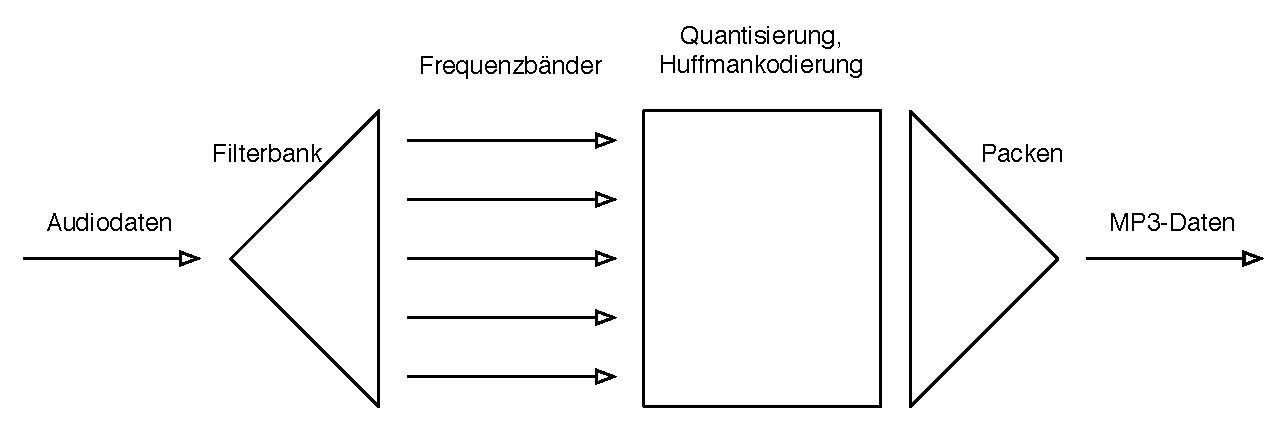
\includegraphics[scale=0.43]{mp3-kodierung3}
  \caption{MP3-Kodierungsverfahren}
  \label{gra:mp3-kodierung}
\end{figure}

Das MP3-Kodierungsverfahren besteht meistens aus 3 Phasen (siehe
Abbildung \ref{gra:mp3-kodierung}):
\begin{enumerate}
\item Als erstes wird eine feste Anzahl an Audiodaten
  (PCM-Audiosamples) der Quelle gefiltert und transformiert. Bei Layer
  1 und Layer 2 werden 384 Samples eingelesen, bei Layer 3 1152
  Samples. Diese Eingangssamples werden durch eine Filterbank in 32
  Fre\-quenz\-b�nder aufgeteilt. Bei Layer 1 und Layer 2 ist dies
  eine einfache Filterbank, bei Layer 3 wird sie durch eine
  hybride Filterbank ersetzt: Die 32 Fre\-quenz\-b�nder werden weiter
  durch eine modifizierte diskrete Kosinustransformation in 18 feinere
  B�nder aufgeteilt, um Redundanzverzerrungen (Maskierungseffekte an
  den Grenzen von Fre\-quenz\-b�ndern) zu vermeiden.
  
\item An Hand dieser transformierten Audiodaten kann der Kodierer mit
  Hilfe eines psychoakustischen Modells bestimmen, wie wichtig
  einzelne Fre\-quenz\-b�nder sind und somit welche Informationsmenge
  ihnen zuzuordnen ist, d.h. mit welcher Aufl�sung sie quantisiert
  werden sollen. Ab Layer 2 kann zu jedem Fre\-quenzband ein
  Skalierungsfaktor angegeben werden, um die Quantisierungsaufl�sung
  anzupassen. Generell werden gr�ssere Werte gr�ber kodiert, kleinere
  Werte daf�r mit h�herer Aufl�sung.  Bei Layer 3 werden die
  Audiodaten anschliessend Huffman-kodiert. F�r die Kodierung werden
  Huffman-Tabellen benutzt, die f�r bestimmte Werteverteilungen
  angepasst sind.
  
  Dieses Verfahren wird iterativ durchgef�hrt, bis ein annehmbarer
  Kompromiss zwischen Qualit�t und Informationsmenge gefunden wurde.
  In einer �usseren Schleife wird jedem Fre\-quenzband ein
  Quantifisierungsfaktor zugewiesen, der solange angepasst wird, bis
  sich das Quantisierungsrauschen unter der Grenze befindet, die durch
  das psychoakustische Modell des Kodierers gesetzt wurde. In einer
  inneren Schleife werden den Audiowerten Huffman-Kodew�rter
  zugewiesen. Wenn die sich daraus ergebende Bitmenge zu gro� ist,
  werden Quantisierung und Skalierung angepasst. Diese Schleifen
  werden solange durchgelaufen, bis der Quantisierungsfaktor aller
  Fre\-quenz\-b�nder angepasst wurde und die resultierende
  Informationsmenge nicht gr�sser als die vorgegebene Bitrate ist.

  Alternativ zu einer festen Ausgangsbitrate kann auch eine variable
  Bitrate benutzt werden. In diesem Fall wird je nach Komplexit�t der
  vorliegenden Audiodaten eine andere Ausgangsbitrate ausgew�hlt, um
  eine feinere Quantisierung der Audiodaten zu erm�glichen.
  
\item Nachdem f�r jedes Fre\-quenzband eine angemessene Quantisierung
  und Kodierung gefunden wurde, m�ssen die kodierten Audiodaten in
  MP3-Frames verpackt werden, damit sie gespeichert und �bertragen
  werden k�nnen. Jedem Frame wird ein Header vorangestellt,
  der die Dekodierungsinformation enth�lt. Das Format des Headers und
  des MP3-Frames wird in dem MP3-Standard bitgenau beschrieben (siehe
  Abschnitt \ref{sec:transcoding}).
\end{enumerate}

\subsection{MP3-Dekodierung}

Das MP3-Dekodierungsverfahren besteht aus der Umkehrung der
Kodierungsschritte, wobei das psychoakustische Analysieren der Eingangsdaten
entf�llt. Die n�tigen Huffmann-Tabellen und Filterkoeffizienten sind
im MP3-Standard festgelegt.
\begin{enumerate}
\item Das anstehende MP3-Frame wird eingelesen und die
  Kodierungsinformationen aus dem Frame-Header extrahiert. An Hand
  dieser Informationen werden die Audiodaten eingelesen.
\item Bei Layer 3 m�ssen die komprimierten Daten
  erst Huffman-dekodiert werden. Aus der Headerinformation wird
  ermittelt, welche Huffman-Tabellen benutzt werden sollen.
\item Anschliessend werden die quantisierten und skalierten Daten
  wieder hergestellt. Die vorliegenden Audiodaten werden durch inverse
  Transformation durch eine synthetisierende Filterbank (bei Layer 3
  noch durch inverse modifizierte diskrete Kosinustransformation) zu
  einem PCM-Signal zur�ckgewandelt.
\end{enumerate}

\subsection{Bit-Reservoir}

Es kann vorkommen, dass ein MP3-Frame sich in weniger Bits als durch
die vorgegebene Bitrate kodieren l�sst. In diesem Fall werden die
unbenutzten Bits in das sogenannte ``Bit-Reservoir'' (siehe Abbildung
\ref{pic:bit-reservoir}) gespeichert.  L�sst sich umgekehrt ein
MP3-Frame nicht ohne Zusatzinformation angemessen kodieren, kann der
Kodierer zus�tzliche Bits aus dem Bit-Reservoir verwenden.

\begin{figure}[htbp]
  \centering
  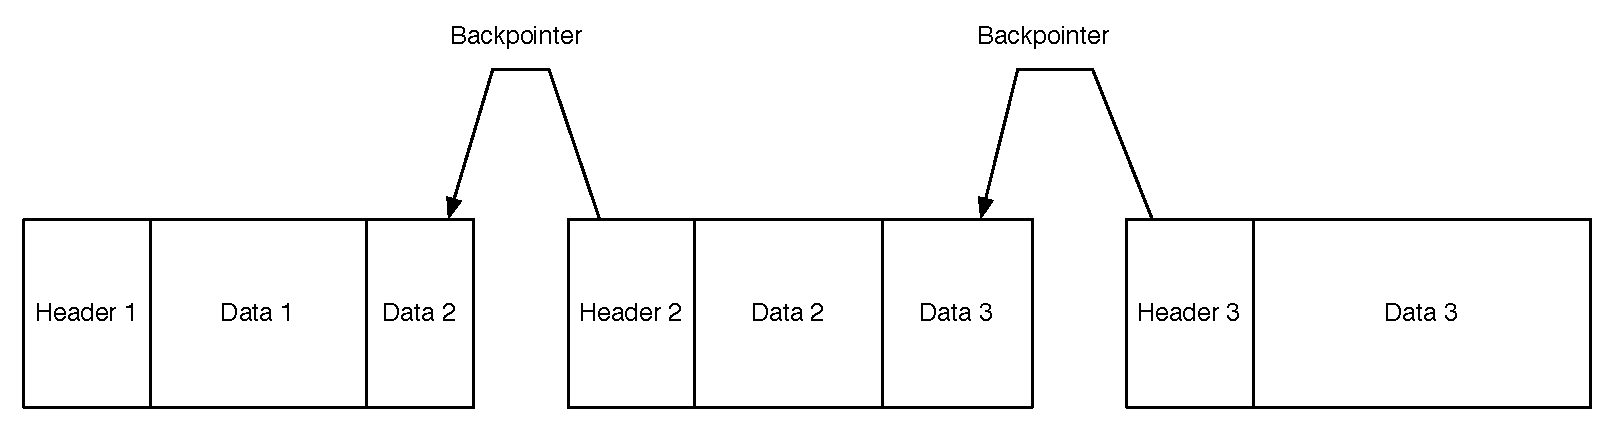
\includegraphics[scale=0.43]{bit-reservoir2}
  \label{pic:bit-reservoir}
  \caption{Bit Reservoir}
\end{figure}

Das Bit-Reservoir wird nicht getrennt gespeichert, sondern direkt in
den MP3-Strom eingef�gt. Das hat zur Folge, dass MP3-Frames nicht mehr
alle zu dem Frame-Header geh�rende Audiodaten beinhalten. Der Anfang
der eigentlichen Audiodaten wird durch einen Verweis auf fr�here Daten
im Strom gegeben (der ``Backpointer''). So kann es vorkommen, dass die
eigentlichen Audiodaten eines MP3-Frames bis zu 9 Frames zur�ck
liegen.

\section{MP3-Streaming}
\label{sec:mp3-streaming}

\subsection{Streaming}

Bei dem Streaming von MP3-Daten werden die Audiodaten als
kontinuierlicher Datenstrom �ber das Netzwerk gesendet, �hnlich wie
bei herk�mmlichen Rundfunkverfahren. Dadurch kann der Benutzer schon
w�hrend der �bertragung der Daten den Inhalt abspielen. Es ist weiterhin
m�glich, mehreren Empf�n\-gern denselben Datenstrom zukommen zu lassen
(``Multicast''), um somit Bandbreite und Netzwerktraffic zu sparen.
Die Netzwerkprogramme (Clients und Server), die im Rahmen dieser
Studienarbeit implementiert wurden, lassen sich sowohl als Unicast-
als auch als Multicastprogramme benutzen (bis auf den HTTP-Streaming
Server).

Das MP3-Format ist f�r Streaming gut geeignet, da zu dem Entschl�sseln
eines MP3-Stromes keine fr�heren Daten notwendig sind (abgesehen vom
Bit-Reservoir). Anders als bei anderen Komprimierungsverfahren, wie
z.B. LZW, ist es nicht notwendig, den Datenstrom von Anfang an zu
entschl�sseln.

\subsubsection{Verfahren}
\label{sub:verfahren}

Wir beschr�nken uns in dieser Arbeit auf ein IP-basiertes Netzwerk.
Die meisten Konzepte lassen sich jedoch auf andere paketorientierte
Netzwerkprotokolle �bertragen.


Audiodaten k�nnen bei IP-Netzwerken in zwei Weisen �bertragen werden:
 \begin{itemize}
 \item Mit dem TCP-Protokoll k�nnen Daten verlustfrei �bertragen
   werden. Korrekt empfangene Pakete (mit korrekter Pr�fsumme) werden
   vom Empf�n\-ger quittiert. Geht allerdings ein Paket verloren,
   entf�llt diese Quittierung, und der Sender sendet das Paket erneut.
   Somit wird gew�hrleistet, dass keine Daten verloren gehen.  Pakete,
   die in falscher Reihenfolge am Ziel ankommen, werden entweder
   verworfen oder umgeordnet. Dieses automatische Neusenden von
   verlorenen Paketen f�hrt allerdings zu Verz�\-ge\-rungen in dem
   Datenstrom.  Bei TCP wird mehr Wert auf die Aufrechterhaltung einer
   kontinuierlichen und verlustlosen Verbindung gelegt, als auf die
   zeitlich nahe Auslieferung der einzelnen Pakete. Es besteht auch
   das Problem, dass TCP nicht f�r Situationen geeignet ist, an der
   mehrere Empf�n\-ger teilnehmen (Broadcast, Multicast).
 \item Mit dem UDP-Protokoll k�nnen Daten als Datagramme fehlerfrei
   versendet werden. Allerdings wird nur gew�hrleistet, dass
   empfangene Pakete korrekt sind; nicht, dass sie am Ziel
   ankommen, und auch nicht, dass sie in der richtigen Reihenfolge
   empfangen werden. Gerade wegen diesem Verzicht auf eine
   verlustfreie End-zu-End-Verbindung ist UDP gut geeignet als
   Transportprotokoll f�r Multicastanwendungen. Ein weiterer Vorteil
   von UDP ist die kleinere Paketheaderl�nge von 8 Bytes, mit der sich
   Audiodaten effizienter versenden lassen.
\end{itemize}
% TCP, UDP, RTP, RTSP

Auf diesen zwei grundlegenden Protokollen bauen weitere Protokolle auf:
\begin{itemize}
  % RFCS f�r HTTP
\item HTTP ist ein auf TCP aufbauendes Anfrage/Antwort Protokoll, dass
  haupt\-s�chlich zur �bermittlung von Webseiten benutzt wird. HTTP hat
  sich auch als MP3-Streaming Protokoll durchgesetzt.  Allerdings
  gelten hier genau dieselben Einschr�nkungen wie f�r TCP, n�mlich
  dass sich das zeitliche Verhalten der �bertragung der Audiodaten
  sehr schlecht ein\-sch�\-tzen l�sst, und das HTTP nicht f�r
  Multicastanwendungen (wie z.B. Internetradio) geeignet ist, da der
  Audiostream zu jedem Empf�n\-ger erneut versendet werden muss.
\item RTP setzt auf UDP auf, und wurde gerade f�r Streaminganwendungen
  konzipiert. Verschiedene RTP-Standards definieren wie
  Multimediadaten in UDP-Pakete verpackt werden sollen. Zus�tzlich
  definiert RTP ein Feedback-Protokoll namens RTCP, mit dem der
  RTP-Server periodische Kontrollanfragen an seine Empf�n\-ger schickt,
  um z. B. die Auslastung der Verbindung abzufragen.  Mit
  diesen Informationen kann der Server dann den Datenstrom anpassen,
  um eine bessere �bermittlung der Daten zu erreichen. In den RFCs
  2250 und 3119 wird beschrieben, wie man MP3-Daten �ber RTP streamen
  kann.
\end{itemize}

\subsubsection{Ver\-z�\-ge\-run\-gen}

Bei einem paketorientierten Netzwerk kann es zu mehreren unerw�nschten
Nebenwirkungen kommen, die die Qualit�t eines Audiodatenstromes
erheblich beeinflussen k�nnen:
\begin{itemize}
\item Aufgrund eines Puffer�berlaufs in einer Netzwerkkomponente
  (Router, Switch) kann es zu Paketverlusten kommen. Einzelne
  verschickte Pakete erreichen nicht ihr Ziel.
\item Es kann zu Ver\-z�\-ge\-run\-gen kommen, und sogar zu eine Umordnung in
  der Paketreihenfolge, wenn einzelne Pakete �ber verschiedene Routen
  weitergeleitet werden.
\end{itemize}

% Delay
% QOS, Buffering
Da das IP-Protokoll keine �bertragungszeiten garantiert, sind
Ver\-z�\-ge\-run\-gen in jedem der in \ref{sub:verfahren} vorgestellten
Verfahren m�glich.  Als Folge dieser Ver\-z�\-ge\-run\-gen kommt es meistens
zu Aussetzern in der Wiedergabe der Audiodaten. Bei radio�hnlichen
Anwendungen l�sst sich dieses Problem durch Puffern der eingehenden
Audiodaten in einen Cache in begrenztem Ma�e l�sen. Allerdings ist das
Puffern von einkommenden Daten in Anwendungsf�llen, die eine
Echtzeit�bertragung der Audiodaten vorraussetzen, wie
Internet-Te\-le\-pho\-nie, nicht m�glich, da eine Verz�gerung bei der
�bertragung von Telefongespr�chen nicht annehmbar ist. Eine andere
M�glichkeit, das Ver\-z�\-ge\-rungs\-pro\-blem zu l�sen, ist die Einf�hrung von
Quality-of-Service-Verfahren.  In einem solchen Fall werden IP-Pakete
verschiedenen Priorit�tsklassen zugeordnet, mit denen die
Router eine verz�gerungsfreie Verbindung gew�hrleisten k�nnen.

Wir setzen in dieser Arbeit eine radio�hnliche Anwendung voraus, und
verwenden keine QOS-Verfahren.

\subsubsection{Paketverluste}
\label{paketverluste}
% Packetloss
Bei der �bertragung der Audiodaten kann es zu einem Verlust der
gesendeten Paketen kommen. Bei bestimmten Anwendungen sind fehlende
Pakete auf Empf�n\-gerseite fatal, weil der Datenstrom nicht mehr
verarbeitet werden kann. MP3 kann allerdings bei dem Verlust von
beliebig vielen Frames weiter entschl�sselt werden, so dass es bei
Paketverlusten nur zu Aussetzern in der Wiedergabe der Audiodaten
kommt.

\begin{figure}[htbp]
  \centering
  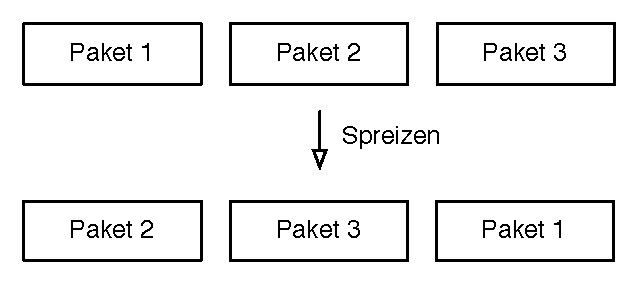
\includegraphics[scale=0.43]{interleaving}
  \label{pic:interleaving}
  \caption{Spreizen von Paketen}
\end{figure}

% Interleaving
Die Korrelation von Paketverlusten kann benutzt werden, um die
Auswirkung von Paketverlusten zu minimieren.  Aufeinanderfolgende
Datengruppen (in unserem Fall MP3-Frames) k�nnen auf nicht
aufeinanderfolgende Pakete ``gespreizt'' werden
(siehe Abbildung \ref{pic:interleaving}). Bei einem Verlust von
mehreren Paketen kommt es dann nicht mehr zu einem langem Aussetzer in
der Wiedergabe, sondern zu mehreren kleinen Unterbrechungen, was f�r
den H�rer wesentlich angenehmer ist.

% FEC
Um eine Verschlechterung des Audiostroms bei Paketverlusten ganz zu
vermeiden, und nicht nur die Aussetzer f�r den H�rer ``angenehmer'' zu
gestalten, k�nnen Daten redundant verschickt werden. Die eleganteste
L�sung ist die Verwendung eines Vorw�rtsfehlerkorrektur-Verfahrens
(Forward Error Correction). Aus $n$ zu versendenden Paketen werden $n
+ k$ Pakete gebildet, die alle �bertragen werden.  Die Empfangsseite
braucht nur $n$ Pakete von den $n+k$ gesendeten Paketen um die
Ursprungsdaten wieder herstellen. In dieser Studienarbeit wird ein
Verfahren beschrieben, mit dem FEC kodierte MP3-Daten �bertragen
werden.  Dieses Verfahren wird ausf�hrlich in den Kapiteln
\ref{sec:transcoding}, \ref{sec:fec} und \ref{sec:implementation}
beschrieben.



\chapter{Streaming-Verfahren f�r MP3-Daten}
\label{sec:streaming}

In diesem Kapitel werden die in Kapitel \ref{sec:uebersicht}
vorgestellten Verfahren analysiert und eine Erweiterung zur
Verbesserung der Sicherheit von RTP-Str�men vorgestellt.  Als erstes
wird das Versenden von MP3-Daten �ber HTTP erkl�rt, dann das in RFC
2250 beschriebene RTP-Protokoll, und schliesslich das in RFC-3119
beschriebene RTP-Protokoll.

\section{HTTP Streaming}

Das HTTP-Streaming von MP3-Daten verwendet die Eigenschaft von
MP3-Dekodierern, unvollst�ndige MP3-Dateien abspielen zu k�nnen. Die
MP3-Daten werden wie eine normale Datei �ber HTTP �bermittelt, und bei
Empfang sofort dekodiert und wiedergeben. Um Metainformationen zu
�bermitteln, wird ein paralleler UDP-Kommunikationskanal
ge�ffnet. �ber diesem Kanal werden die Informationen gesendet, die in
den ID3-Tags am Ende der MP3-Datei stehen.

HTTP-Streaming ist einfach zu implementieren, weil die
Synchronisation zwischen Quelle und Empf�nger durch die
TCP-Verbindungsschicht des Betriebssystems �bernommen wird. Die
TCP-Flu�kontrollmechanismen regulieren dann die Sendegeschwindigkeit.
Im Rahmen dieser Arbeit wurde ein HTTP-MP3-Streaming Server
implementiert (siehe \ref{impl:poc-http}).

\section{RTP Streaming}

\subsection{�bersicht: RTP}
RTP wird in RFC-1889 als Protokoll zur
�bermittlung von Multimediadaten definiert. RTP wird meistens �ber UDP
verwendet, stellt allerdings selber keine Mechanismen zur Verf�gung,
um Paketverluste zu vermeiden oder Quality of Service zu sichern. RTP
ist sozusagen ein ``Baustein''-Protokoll, das je nach Anwendungsfall
erweitert werden muss. Durch das unterliegende UDP-Protokoll ist RTP
sowohl in Unicast- als auch in Multicast-Anwendungsf�llen
einsetzbar. So wird RTP z.B. bei Audio- und Video-Konferenzen �ber
Internet oder Satellitverbindungen eingesetzt.

Jedes RTP-Paket besteht aus einem RTP-Header, weiterhin einem
sogenannten ``erweiterten'' Header und den Anwendungsdaten.  Das
Format des erweiterten Headers sowie die Bedeutung einzelner Bits im
normalen RTP-Header werden in RFC-1889 nicht beschrieben, sondern
m�ssen je nach Anwendungsfall angegeben werden.

Im RTP-Header k�nnen Anwendungsdaten mit einem
Datentyp\-mar\-kie\-rungs\-feld, einem Timestampfeld und einer Sequenznummer
sowie Quellinformationen versehen werden. Die Quellinformationen
werden benutzt, um verschiedene RTP-Sitzungen zu beschreiben. Diese
RTP-Sitzungen erm�glichen einen Wechsel der Kodierung, und erlauben
das Ver�ndern der Anwendungsdaten durch Zwischenknoten (sogenannte
``Translator''-Knoten).
\begin{figure}[htbp]
  \centering
  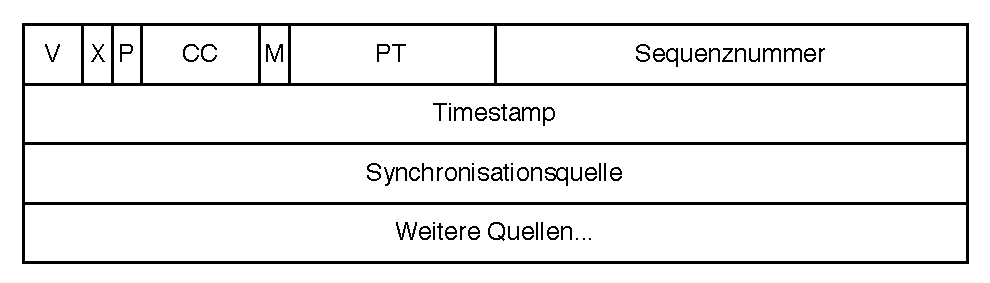
\includegraphics[scale=.43]{rtp2}
  \label{pic:rtp}
  \caption{Format des RTP-Headers}
\end{figure}
Die Felder in Abb. \ref{pic:rtp} haben folgende Bedeutung:
\begin{description}
\item[V:] RTP-Versionsnummer
\item[P:] Paddingbit, um Zusatzdaten am Ende des RTP-Pakets speichern
  zu k�nnen
\item[X:] Erweiterungsbit, um einen erweiterten Header hinter dem
  normalen RTP Header speichern zu k�nnen
\item[CC:] Anzahl der Zusatzquellen am Ende des Headers
\item[M:] Markerbit, anwendungsspezifisch zu interpretieren
\item[PT:] Anwendungstyp der RTP-Daten. Anwendungstype
  werden in weiteren Dokumenten beschrieben.
\end{description}

Zus�tzlich zum RTP-Paketformat definiert RFC-1889 auch RTCP
(\emph{Real-Time Control Protocol}), mit dem Empf�nger Informationen
an die RTP-Quelle zu\-r�ck\-sen\-den k�nnen. An Hand dieser Information kann
die RTP-Quelle die Paketverlustrate und Verz�gerungszeiten f�r
einzelne Empf�ngerknoten berechnen, und den RTP-Strom
anpassen. Allerdings scheint das RTCP-Protokoll kaum benutzt zu
werden. In den RTP-Implementierungen dieser Arbeit wird RTCP nicht
ber�cksichtigt.

\subsection{RFC-2250 Streaming}

In RFC-2250 wird beschrieben, wie MP3-Daten �ber RTP
zu versenden sind. Jedes MP3-Frame wird in ein RTP-Paket verpackt:
\begin{itemize}
\item die Sequenznummer in dem RTP-Header wird auf die Nummer des
  Frames innerhalb der MP3 Datei gesetzt. Ein Dateiwechsel wird durch
  das Setzen des Markerbits im Header signalisiert.
\item Der Timestamp wird aus der 90 kHz Uhr des MP3-Systems
  berechnet. Dieser Timestamp wird nicht beim Dekodieren
  der MP3-Daten ber�ck\-sich\-tigt, sondern dient nur der Synchronisation
  des Empf�ngers, um Netzwerkverz�gerungen zu korrigieren.
\item Das Anwendungstypfeld wird auf 14 gesetzt.
\end{itemize}

In einem RTP-Paket k�nnen mehrere MP3-Frames gespeichert werden.  Es
kann allerdings vorkommen, da� ein einzelnes MP3-Frame die maximale
Gr�sse eines RTP-Pakets �berschreitet, so da� dieses Frame
fragmentiert werden muss.  In diesem Fall wird ein erweiterter Header
benutzt, der Fragmentierungsinformation beinh�lt:
\begin{figure}[htbp]
  \centering
  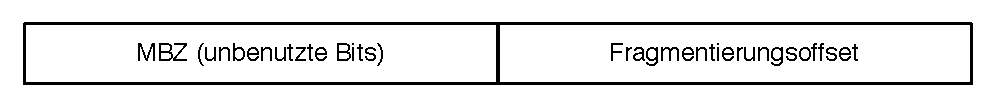
\includegraphics[scale=.43]{rtp2250-2}
  \label{pic:rtp2250}
  \caption{Format des erweiterten RFC-2250 Headers}
\end{figure}
\begin{description}
\item[Fragmentierungsoffset:] Gibt den Offset der RTP-Anwendungsdaten
  in dem derzeitigen MP3-Frame an.
\end{description}

Die Sequenznummer des RTP-Headers erm�glicht es, Umordnungen bei der
Reihenfolge der Pakete zu beheben. In unserer Implementierung wird ein
Paketpuffer benutzt, um eintreffende Pakete dem MP3-Dekodierer in der
richtigen Reihenfolge zu �bergeben.

\subsection{RFC-3119 Streaming}

In RFC-2250 stimmen RTP-Paketgrenzen mit MP3-Frames
�berein. Audiodaten zu einem MP3-Frame k�nnen aber in dem
Bit-Reservoir gespeichert sein, also in einem vorigen Frame. Deswegen
sind MP3-Frames keine unabh�ngigen Dateneinheiten (ADU,
\emph{Application Data Unit}).  Ein verlorenes RTP-Paket kann also
gro�e Auswirkungen auf den MP3-Strom haben, weil Teile des
Bit-Re\-ser\-voirs f�r sp�tere Frames fehlen k�nnten.

In RFC-3119 wird ein neues RTP-Format beschrieben, in dem nicht mehr
MP3-Frames als RTP-Anwendungsdaten verschickt werden, sondern
ADU-Frames. Ein ADU-Frame wird als ein MP3-Header und die
dazugeh�rigen Audiodaten definiert, ob diese Audiodaten nun im
Bitreservoir zu finden sind, oder im ``normalen'' MP3-Frame, der zum
MP3-Header geh�rt.

Ein RFC-3119-RTP-Paket setzt sich aus einem RTP-Header, einem
erweiterten RTP-Header und einem ADU-Frame zusammen. Das
Markierungsbit im RTP-Header keine Rolle mehr, der Timestamp wird wie
bei RFC-2250 gesetzt. Ist ein ADU Frame gr�sser als die durch das
unterliegende Protokoll zugelassene maximale Paketgr��e sein, so wird
das Paket fragmentiert: das Continuation-Flag des erweiterten RTP
Headers signalisiert, da� die RTP Anwendungsdaten Teil eines
vorherigen ADU Frames sind.  Bei dem erweiterten Header kann die
Gr�sse in 6 bits f�r ADU Frames die kleiner als 64 Bytes sind, oder 14
bits f�r gr�ssere ADU Frames angegeben werden.

% interleaving
RFC-3119 erm�glicht das Spreizen von Paketen (siehe
\ref{paketverluste}).  Dazu werden die 11 h�heren Bits des MP3
Synchronisationswortes (siehe \ref{mpeg:headerformat}) in einen 8 Bits
langen Spreizungsindex und einen 3 Bits langen Spreizungszyklus-Z�hler
unterteilt (Abb. \ref{pic:rtp3119interleaving}).
\begin{figure}[htbp]
  \centering
  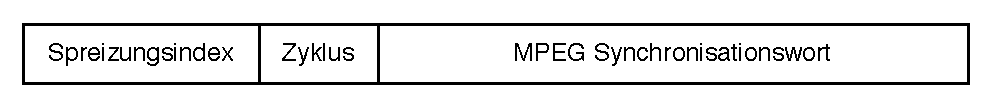
\includegraphics[scale=0.43]{rtp3119c-2}
  \label{pic:rtp3119interleaving}
  \caption{Unterteilung des MP3-Synchronisationswortes}
\end{figure}
Der Spreizungszyklusz�hler wird benutzt, um gepufferte Pakete am Ende
eines Zyklus an den MP3-Dekodierer weiterzugeben: an dem
Zeitpunkt werden meistens keine Pakete der jetzigen Spreizungsgruppe mehr
empfangen.

% implementierung
In der Implementierung (Abb. \ref{pic:rfc3119impl}) von RFC-3119 wird
der im RFC angegebene Konvertierungsalgorithmus benutzt. Der Sender
liest solange MP3-Frames ein, bis ein komplettes ADU-Frame erzeugt
werden kann. Das fertige ADU-Frame wird zwischengespeichert, damit
sp�ter mehrere ADU-Frames auf verschiedene RTP Pakete
gespreizt werden. Nach dem Bilden einer kompletten Spreizungsgruppe
werden die umsortierten Pakete verschickt.

\begin{figure}[htbp]
  \centering
  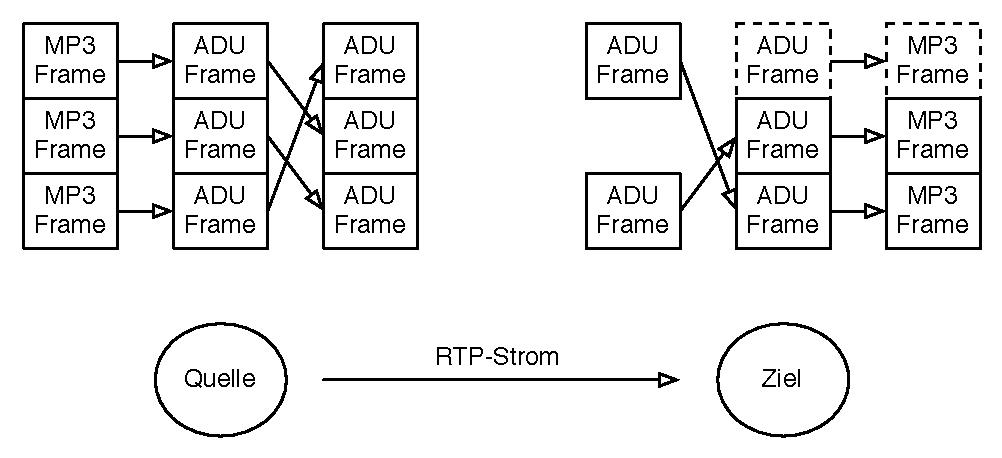
\includegraphics[scale=0.43]{rfc3119impl}
  \label{pic:rfc3119impl}
  \caption{Funktionsweise von RFC-3119}
\end{figure}

Der Empf�nger liest solange Daten, bis eine Spreizungsgruppe empfangen
wurde. Zu jedem ADU-Frame wird das urspr�ngliche MP3-Frame wieder
hergestellt (es sei denn, der MP3-Dekodierer kann ADU-Frames direkt
dekodieren).  Falls es bei der �bertragung zu Paketverlusten kam
k�nnen MP3-Frames nicht mehr ``gef�llt'' werden, weil die
Bitreservoirinformation der verlorenen ADU Frames fehlt. In diesem
Fall wird die L�cke mit Nullen gef�llt, und es wird ein leeres
ADU-Frame eingef�gt (mit leerem MP3 Header), damit der MP3-Strom
korrekt dekodierbar bleibt.

\subsection{Sicherheit von RTP Streaming}
\label{sec:rtp-sec}

Beide RTP Streamingverfahren leiden an einem grundlegendem
Sicherheitsproblem. Bei UDP ist es erheblich einfacher als bei TCP,
Datenpakete zu f�lschen. Das f�hrt im besten Fall zu einem
Zusammenbruch des Datenstroms, weil der Dekodierer mit der sinnlosen
Information nicht zurecht kommt, im schlimmsten Fall wird die
Kommunikation von dem unberechtigten Partner �ber\-nom\-men.

\begin{figure}[htbp]
  \centering
  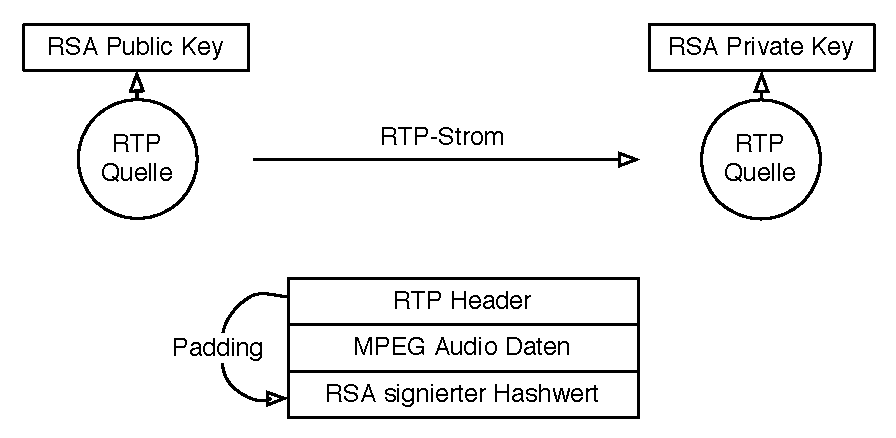
\includegraphics[scale=0.43]{rtprsa2}
  \label{pic:rtprsa}
  \caption{RSA Signierung von RTP Anwendungsdaten}
\end{figure}

Wenn jedes Datenpaket mit einem Public-Key Verfahren kryptographisch
signiert wird, kann der Empf�nger mit dem �ffentlichen Schl�ssel der
Quelle die G�ltigkeit der Daten �berpr�fen (siehe Abbildung
\ref{pic:rtprsa}). Bei der Implementierung dieser Studienarbeit werden
die Hashwerte der Datenpakete mit RSA signiert, der signierte Hashwert
wird als Padding an das Ende von jedem RTP Paket angeh�ngt. Somit
k�nnen auch herk�mmliche RTP Implementierungen die signierten Pakete
dekodieren. Attacken durch erneutes Senden von abgeh�rten Paketen
werden vermieden, weil der Empf�nger schon empfangene Pakete verwirft.

\section{Streaming mit Fehlerkorrektur}

Bei RFC-3119 werden die Auswirkungen von Paketverlusten gegen�ber
RFC-2250 minimiert, verlorene Pakete f�hren nachwievor zu Aussetzern
in dem MP3-Strom. Im Rahmen dieser Studienarbeit wurde ein Verfahren
entwickelt, bei dem ADU-Frames mit dem FEC-Verfahren von Luigi Rizzo
\cite{FEC} redundant kodiert werden (siehe
Abb. \ref{pic:fecimpl}). Bei Paketverlusten k�nnen aus den redundant
kodierten Paketen die Quelldaten wiederhergestellt werden.

\begin{figure}[htbp]
  \centering
  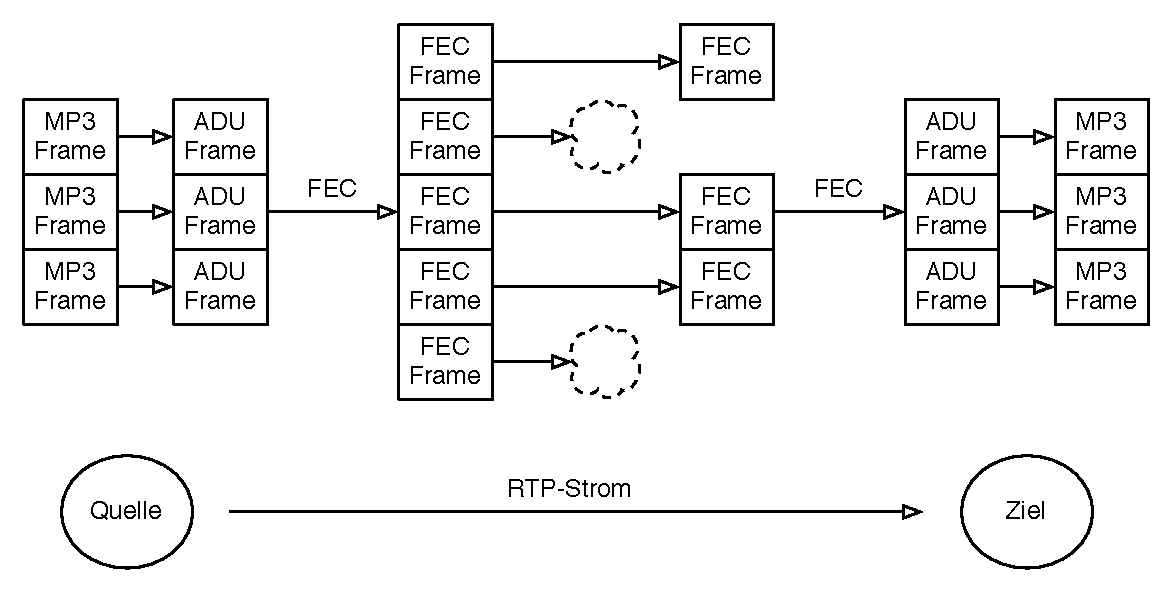
\includegraphics[scale=.43]{fecimpl}
  \label{pic:fecimpl}
  \caption{Funktionsweise von FEC Streaming}
\end{figure}


\chapter{Verarbeitung von MP3-Daten}
\label{sec:transcoding}

Wegen der Frameabh�ngigkeiten, die durch das Bitreservoir entstehen,
werden bei Paketverlusten bei RFC-2250 gleich mehrere Frames unlesbar,
weil das zu dem MP3-Header geh�rige Bitreservoir nicht vorhanden ist.
MP3-Frames m�ssen vor dem Senden zu unabh�ngigen Dateneinheiten (ADUs)
zusammengesetzt werden, damit Paketverluste keinen
frame-�bergreifenden Einfluss auf den MP3-Strom haben.

In diesem Kapitel wird zuerst die Struktur eines MP3-Stromes
erl�utert. Anschliessend werden die Algorithmen vorgestellt, mit denen
MP3-Frames zu ADUs und ADUs wieder zur�ck in MP3-Frames konvertiert
werden.

\section{Einlesen von MP3-Frames}

% Format von MP3 Frames
\subsection{Format eines MP3-Headers}
\label{mpeg:headerformat}

% Headerformat
Ein MP3-Header ist 4 Bytes lang (siehe Abbildung
\ref{pic:mp3hdr}). Die 12 ersten Bits dienen als Synchronisationswert.
Dieser Synchronisationswert wird von Layer, Bitrate, Samplerate und
Stereokodierungsmodus (normale Stereokodierung, Joint Stereo oder
Einkanalkodierung) gefolgt. Bei Layer 3 wird der MP3-Header von
zus�tzlicher Information erg�nzt, die in der
Nebensinformationsstruktur (\emph{Sideinformation structure})
gespeichert ist (siehe Abbildung \ref{pic:mp3si}).

\begin{figure}[htbp]
  \centering
  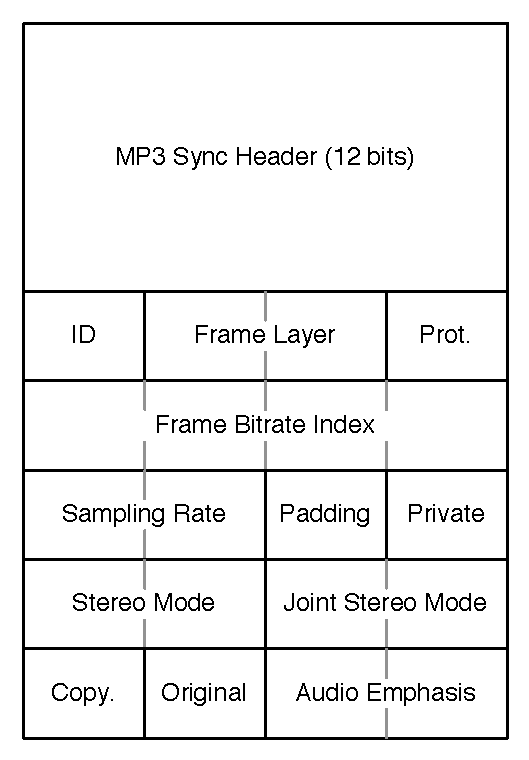
\includegraphics[scale=0.43]{mp3hdr}
  \label{pic:mp3hdr}
  \caption{MP3-Header}
\end{figure}

Diese zus�tzliche Information gibt den Anfangsindex des Bit-Reservoirs
an (der ``Backpointer'', der angibt, wieviele Bytes des jetzigen
MP3-Frames in vorigen Frames zu finden sind), und ob
Skalierungsfaktoren innerhalb eines Frames wiederbenutzt werden
k�nnen.  Kodierungsinformationen f�r die eigentlichen Audiodaten sind
auch in der Nebeninformationsstruktur gespeichert.  Diese
Kodierungsinformation ist in Stereokan�le (2 bei Stereokodierungen, 1
bei Einkanalkodierung) eingeteilt, welche wiederrum in 2 Einheiten
eingeteilt sind, die ``Granules'' genannt werden. In dieser
Granule-Information wird die Aufl�sung der Skalierungsfaktoren f�r den
Frequenzspektrum angegeben, die Windowinginformation f�r die
Aliasreduktion bei der Synthese der Audiodaten sowie die
Tabellenangaben f�r die Huffmandekodierung der komprimierten
Audiodaten gespeichert.

\begin{figure}[htbp]
  \centering
  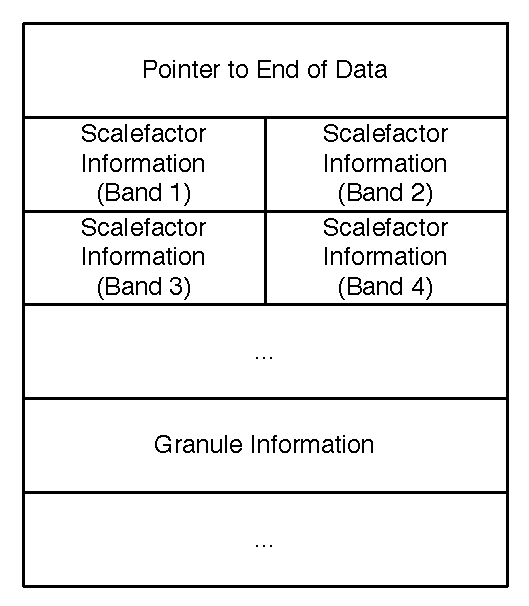
\includegraphics[scale=0.43]{mp3si}
  \label{pic:mp3si}
  \caption{MP3-Header Nebeninformation}
\end{figure}

\subsection{Transformierung nach ADUs}
\label{sec:aq}
Bevor die eigentlichen Audiodaten zu einem MP3-Header eingelesen
werden k�nnen muss Information aus dem Bitreservoir in fr�heren
MP3-Frames zusammengesetzt werden, um ein ADU (eine alleinstehende
Informationseinheit) zu bilden (siehe Abbildung
\ref{pic:mp3adu}). Dazu wird eine Kettendatenstruktur (``Queue'')
benutzt, in die MP3-Frames eingespielt werden.

\begin{figure}[htbp]
  \centering
  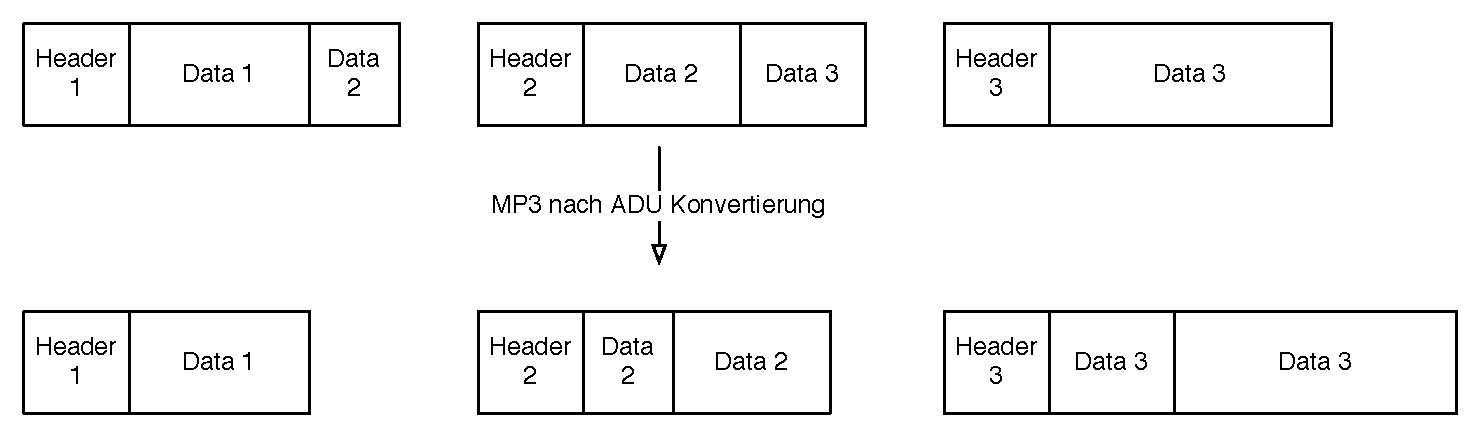
\includegraphics[scale=0.43]{mp3adu2}
  \label{pic:mp3adu}
  \caption{Konvertierung von MP3-Frames nach ADUs}
\end{figure}

Algorithmus A (siehe \ref{alg:A}) bestimmt, ob mit einem neuen
MP3-Frames in der Queue ein ADU generiert werden kann.  ADUs f�r
�ltere Frames k�nnen nicht mehr generiert werden, da die n�tige
Bit-Reservoir-Information nicht mehr vorhanden ist. Mit Algorithmus B
(siehe \ref{alg:B}) wird der Anfang der Audiodaten f�r das neue ADU
bestimmt. �ltere Frames, die keine Teile dieser Audiodaten enthalten,
werden nicht mehr gebraucht und werden freigegeben.  Anschliessend
wird mit Algorithmus C (siehe \ref{alg:C}) das ADU hergestellt.

\begin{figure}[htbp]
  \center{
    \begin{algorithm}
    \item[A1:] \emph{[Einspielen eines neuen Frames]} $A \leftarrow$ Gr��e der
      MP3 Information in der MP3 Frame Kette vor dem
      Einspielen des neuen MP3 Frames
    \item[A2:] Einspielen des neuen MP3 Frames in die Kette
    \item[A3:] $B \leftarrow$ Gr��e der MP3 Information in der
      Kette nach dem Einspielen des neuen MP3 Frames
    \item[A4:] \emph{[Nachpr�fen, ob genug Daten f�r ein neues ADU vorhanden
      sind]} Falls der Backpointer des neuen Frames $> A$, oder $B <$
      Gr��e des ADUs f�r das neue Frame, dann gibt es nicht gen�gend
      Information, um ein ADU zu generieren
    \end{algorithm}}

  \caption{Algorithmus A: Pr�fen, ob gen�gend MP3 Frames in der
Queue vorhanden sind, um ein neues ADU zu generieren}
  \label{alg:A}
\end{figure}

% XXX Bild zu algorithmus A mit Backpointer und L�nge der einzelnen Frames

\begin{figure}[htbp]
  \center{
    \begin{algorithm}
    \item[B1:] \emph{[Initialisierung]} $A \leftarrow$ Backpointer des neusten Frames
    \item[B2:] \emph{[Ber�cksichtigen des vorigen Frames]} $B \leftarrow$ das
      vorige Frame
    \item[B3:] $A \leftarrow A -$ Framegr��e von $B$
    \item[B4:] \emph{[Pr�fen, ob gen�gend Daten f�r das neue ADU vorhanden
      sind]} Falls $A > 0$, gehe nach {\bf B2}
    \item[B5:] \emph{[Ermitteln des Anfangs des neuen ADUs]} Das erste Frame,
      was Daten f�r das neue ADU beinh�lt ist $B$, $-A$ ist das Offset
      innerhalb von $B$, an dem diese Daten anfangen.
    \end{algorithm}}
    
  \caption{Algorithmus B: Bestimmen des Anfangs der Audiodaten}
  \label{alg:B}
\end{figure}

\begin{figure}[htbp]
  \center{
    \begin{algorithm}
    \item[C1:] \emph{[Initialisierung]} $A \leftarrow$ erste Frame, da� Daten
      des neuen ADUs enth�lt \\
      $B \leftarrow$ Offset innerhalb von $A$, an
      dem die Daten des neuen ADUs anfangen \\
      $C \leftarrow$ Gr��e des neuen ADUs
    \item[C2:] \emph{[Kopieren der Daten in das neue ADU]} $D \leftarrow$
      Gr��e von $A - B$
    \item[C3:] $E \leftarrow$ Minimum von $D$ und $C$
    \item[C4:] Kopiere $E$ von $A$ an Offset $B$ in das neue
      ADU
    \item[C5:] \emph{[Einspielen des n�chsten Frames]} $C \leftarrow C - E$,
      $A \leftarrow$ n�chstes Frame in der Kette, $B \leftarrow 0$
    \item[C6:] Falls $C > 0$, dann gehe nach {\bf C2}
    \end{algorithm}}
  
  \caption{Algorithmus C: Herstellen des neuen ADUs}
  \label{alg:C}
\end{figure}

\subsection{Konvertierung von ADUs nach MP3-Frames}

Wenn der MP3-Dekodierer nicht mit ADUs umgehen kann, m�ssen die ADUs
zur�ck in ``normalen'' MP3-Frames transformiert werden.  Analog zur
Konvertierung von MP3-Frames in ADUs wird auch hier eine
Kettendatenstruktur verwendet, in die ADUs eingespielt werden.
Algorithmus D (siehe \ref{alg:D}) pr�ft nach, ob gen�gend ADUs in der
Kette vorhanden sind, um ein MP3-Frame f�r das erste ADU zu
generieren.  Sind gen�gend ADUs vorhanden, generiert Algorithmus
E (siehe \ref{alg:E}) das MP3-Frame f�r das erste ADU in der Queue.

\begin{figure}[htbp]
  \center{
    \begin{algorithm}
    \item[D1:] \emph{[Initialisierung]} $A$ (Gr��e des zu generienden MP3 Frames)
      $\leftarrow$ Gr��e des MP3 Frames f�r das erste ADU
      in der Kette, $B$ (Gr��e des vorherigen MP3 Frames)
      $\leftarrow 0$, $C$ (durchl�uft die ADUs in der Kette)
      $\leftarrow$ erstes ADU in der Kette
    \item[D2:] $D$ (Ende der Audiodaten, die in $C$ enthalten
      sind) $\leftarrow$ Gr��e von $C -$ Backpointer von $C + B$
    \item[D3:] \emph{[Pr�fen, ob gen�gend Daten f�r das neue MP3 Frame
        vorhanden sind]} Falls $D > A$, dann ist gen�gend Information
      vorhanden, um ein MP3 Frame f�r das erste ADU in der
      Kette zu generieren \item[D4:] $B \leftarrow B +$ Gr��e des MP3
       Frames von $C$
    \item[D5:] \emph{[Pr�fen, ob weitere ADUs vorhanden sind]} Falls
      keine ADUs mehr in der Kette vorhanden sind, dann kann kein MP3
       Frame f�r das erste ADU generiert werden, sonst $C
      \leftarrow$ n�chstes ADU in der Kette
    \item[D6:] Gehe zu {\bf D2}
    \end{algorithm}}

  \caption{Algorithmus D: Pr�fen, ob gen�gend ADUs in der Queue
    vorhanden sind}
  \label{alg:D}
\end{figure}

\begin{figure}[htbp]
  \center{
    \begin{algorithm}
    \item[E1:] \emph{[Initialiserung des neuen MP3 Frames]} Kopiere
      den MP3 Header und die zus�tzliche Information
      (``sideinfo'') des ersten ADUs in der Kette in das neue MP3
       Frame, f�lle die MP3 Daten des neuen Frames mit $0$
    \item[E2:] \emph{[Initialisierung]} $A \leftarrow$ erstes ADU in
      der Kette, $B$ (Index der Audiodaten in vorherigen ADUs)
      $\leftarrow 0$, $C \leftarrow$ Gr��e des zu generierenden MP3
       Frames
    \item[E3:] \emph{[Berechnen des Anfangs des neuen MP3 Frames]} $D$
      (Anfang der Audiodaten in $A$ relativ zu dem Anfang der Daten in
      dem zu generierenden MP3 Frame) $\leftarrow$ $A -$
      Backpointer von $A$
    \item[E4:] Falls $D > C$, dann gehe zu E10
    \item[E5:] $E$ (Ende der Audiodaten in $A$ relativ zu dem
      Anfang der Daten in dem zu generienden MP3 Frame) $\leftarrow$
      max($D$ + Gr��e von $A$, $C$)
    \item[E6:] \emph{[Berechnen der Datenoffsets]} Falls $D < 0$, dann
      $F$ (Anfangsindex der Audiodaten innerhalb des ADUs)
      $\leftarrow$ - $D$, $G$ (Zielindex der Audiodaten innerhalb des
      zu generierenden MP3 Frames) $\leftarrow$ 0 und $H$
      (Gr��e der zu kopierenden Audiodaten) $\leftarrow E$. Sonst $F
      \leftarrow$ 0, $G \leftarrow D$ und $H$ $\leftarrow E - D$
    \item[E7:] \emph{[Kopieren der Daten des neuen Frames]} Kopiere
      $H$ Bytes aus den Audiodaten von $A$ ab Index $F$ an Index $G$
      in den zu generierenden MP3 Frame
    \item[E8:] $B \leftarrow B +$ Gr��e des MP3
      Frames von $A$
    \item[E9:] \emph{[Einspielen des n�chsten ADUs]} Falls $E < C$,
      dann $A \leftarrow$ n�chstes ADU in der Kette und gehe zu {\bf
        E3}
    \item[E10:] \emph{[L�schen des dekodierten ADUs]} L�sche das erste
      ADU aus der Kette
    \end{algorithm}}

   \caption{Algorithmus E: Generieren des MP3-Frames}
   \label{alg:E}
\end{figure}

Beim Einspielen von ADUs in die Queue kann es vorkommen, da� der
Backpointer des neu eingespielten ADUs mit den Audiodaten des
vorherigen ADUs �berlappt. Das bedeutet, da� ADUs verloren gegangen
sind, in welchem Fall leere ADUs eingespielt werden, um eine korrekte
Queue wiederherzustellen. Dieses Verfahren ist allerdings nur dann
notwendig, wenn der MP3-Dekodierungsprozess nicht gesteuert werden
kann (z.B. wenn der MP3-Dekodierer ein getrenntes Programm ist, das nicht
ver�ndert werden kann, und die dekodierten ADU Daten als Datenstrom
bekommt). Sonst kann der MP3-Dekodierer bei fehlenden ADUs einfach eine
Pause einf�gen.



\chapter{Vor\-w�rts\-feh\-ler\-kor\-rek\-tur}
\label{sec:fec}

In diesem Kapitel wird ein Verfahren vorgestellt, mit dem
Paketverluste durch \emph{Vor\-w�rts\-feh\-ler\-kor\-rek\-tur} (``Forward Error
Correction'') ausgeglichen werden. Vor\-w�rts\-feh\-ler\-kor\-rek\-tur\-verfahren
werden meistens von allgemeineren Fehlerkorrekturverfahren abgeleitet,
die auch Sendefehler korrigieren k�nnen. In unserem Fall (Senden �ber
IP) werden Sendefehler durch die unterliegenden Netzwerkschichten
schon behandelt, so dass wir uns nur noch um Paketverluste k�mmern
m�ssen.  Hier kommen sogenannte \emph{Block Erasure Codes} zum
Einsatz. Wir setzen das von Rizzo in \cite{FEC} beschriebene Verfahren
ein, welches sich effizient in Software implementieren l�sst.

\section{Ein lineares, systematisches Verfahren}

\subsection{Lineare, systematische Codes}
% Lineare Codes
Bei Fehlerkorrekturverfahren, die Paketverluste ausgleichen, werden
$k$ Quelldatenpakete in $n$ ($n > k$) kodiert, und $n$ Pakete
anschliessend versendet. $k$ empfangene Pakete sind ausreichend, um
die Quelldaten wieder herzustellen. Das Verfahren von Rizzo l�sst sich
in die Klasse der \emph{linearen Fehlerkorrekturcodes}
einordnen. Dabei werden die $k$ Quellpakete ($\overrightarrow{x} = x_0
\ldots x_{k-1}$) an eine $n \times k$ Kodierungsmatrix $G$
multipliziert, um den zu sendenden Paketvektor $\overrightarrow{y}$ zu
erhalten:
\begin{displaymath}
  \overrightarrow{y} = G \overrightarrow{x}.
\end{displaymath}
Damit die empfangenen Pakete aus $\overrightarrow{y}$ wieder zu den
Quellpaketen konvertiert werden k�nnen muss jede Untermatrix von $G$,
die $k$ Zeilen hat, invertierbar sein. Die Matrix $G$ wird auch
\emph{Generatormatrix} genannt.

% Systematische Codes
Weiterhin kann ein Fehlerkorrekturverfahren \emph{systematisch} sein,
wenn die unver�nderten Quelldaten in dem Ergebnisvektor zu
finden sind, also
\begin{displaymath}
  x_0 \ldots x_{k-1} \in \overrightarrow{y}.
\end{displaymath}
Das l�sst sich am einfachsten realisieren, wenn die Identit�tsmatrix
$I_k$ eine Untermatrix von $G$ ist. Ein systematisches
Fehlerkorrektursverfahren hat den Vorteil, dass bei geringem
Paketverlust die Quelldaten mit geringem Berechnungsaufwand
wiederhergestellt werden k�nnen.

% Wiederhergewinnen von Quelldaten
Wenn $k$ Pakete aus $\overrightarrow{y}$ ($\overrightarrow{y'}$)
empfangen werden k�nnen die $k$ Quellpakete wiederhergestellt werden,
indem das Inverse der $G'$ Matrix, die aus den $k$ Gleichungen zu den
Paketen aus $\overrightarrow{y}$ besteht, an $\overrightarrow{y'}$
multipliziert wird:
\begin{displaymath}
  \overrightarrow{y'} = G' \overrightarrow{x} \leftrightarrow
  \overrightarrow{x} = G'^{-1} \overrightarrow{y'}.
\end{displaymath}
Um die Matrix $G'$ zu berechnen muss die Sequenznummer der gesendeten
Pakete bekannt sein, damit es nicht zu fatalen Umordnungen
kommt. Meistens wird diese Information schon durch den unterliegenden
Kommunikationskanal zur Verf�gung gestellt (in unserem Fall durch ein
Feld in dem Paketheader der gesendeten Datenpakete).

% Grafik einfuegen

\subsection{Galoisfeldarithmetik}
% Benutzen von Galoisfeld zur Darstellung der Daten damit keine
 % erhoehte Aufloesung benutzt werden muss.

Wenn die Quelldaten (also $x_i, 0 \leq i < n$) mit $b$ Bits kodiert
werden, und die Elemente der Kodierungsmatrix $G$ mit $b'$ Bits,
m�ssen die Ergebnisse der Kodierungsmultiplikation $G
\overrightarrow{x}$ mit $b + b'$ kodiert werden, um die Genauigkeit zu
% XXX Stimmt das mit b + b'?
erhalten. Der zus�tzliche Datenaufwand ist bei dem Einsatzgebiet des
Verfahrens nicht vertretbar (Verdoppelung der zu sendenden Daten).

Wenn jedoch in einem \emph{endlichen K�rper} gerechnet wird, sind die
Ausgangswerte mit derselben Anzahl Bits kodierbar wie die
Eingangselemente (ein endlicher K�rper ist unter Addition und
Multiplikation geschlossen). In dem Verfahren von Rizzo werden
Galoisk�rper (auch Erweiterungsk�rper) eingesetzt.

\emph{Primk�rper} sind endliche K�rper mit $p$ Elementen, wo $p$
Primzahl ist, und werden $GF(p)$ notiert. Addition und Multiplikation
in einem Primk�rper sind Addition und Multiplikation modulo
$p$. Da Primk�rper sich nur ineffizient implementieren lassen (mit
Ausnahme von $p = 2$ gehen immer Bits bei der Kodierung von Elemente
in $GF(p)$ verloren) werden \emph{Erweiterungsk�rper} eingesetzt, die
$p^r$ Elemente haben und $GF(p^r)$ notiert werden. Elemente aus
$GF(p^r)$ kann man auch als Polynome des Grades $r-1$ �ber $GF(p)$
auffassen. Addition ist die koeffizientenweise Addition modulo $p$,
Multiplikation die Polynommultiplikation modulo einem Minimalpolynom
in $GF(p^r)$ (ohne Teiler in $GF(p^r)$). In jedem Galoisk�rper $G$ existiert
ein \emph{Generatorelement} $\alpha$, das mit sich selbst
multipliziert alle nicht-null Elemente aus $G$ spannt (also $\alpha^0,
\alpha^1, \ldots, \alpha^{p^r}$). Jedem Element $x \in G$ kann man also
den $\alpha$-Logarithmus $k$, so dass $\alpha^k = x$, zuweisen.

Die Operationen in $GF(p^r)$ lassen sich f�r $p = 2$ extrem effizient
implementieren, da Addition sich durch $XOR$ und Multiplikation sich durch
Logarithmuslookuptabellen implementieren lassen.

\subsection{Erstellen der Generatormatrix $G$}

Die $n \times k$ Generatormatrix $G$ muss 2 Bedingungen erf�llen:
\begin{itemize}
\item Jede Untermatrix von $G$ aus $k$ Zeilen muss invertierbar sein,
  damit die Dekodierungsmatrix $G'^{-1}$ auch berechnet werden kann.
\item Die Matrix $G$ muss die $k \times k$ Identit�tsmatrix enthalten,
  damit das Fehlerkorrekturverfahren auch systematisch ist.
\end{itemize}
Um eine solche Matrix zu generieren wird zuerst eine $k \times n$
Vandermonde Matrix erstellt, so dass die erste Zeile Potenzen von $0$
beinhaltet. Die obere $k \times k$ Matrix wird invertiert und an die
untere $k \times (n - k)$ Matrix multipliziert. Die obere $k \times k$
Matrix wird dann mit der $k \times k$ Identit�tsmatrix gef�llt. Damit
ist gew�hrleistet, dass die Generatormatrix korrekt und systematisch ist.
% XXX Klaeren was der Voodoo ist.

\subsection{Kodieren von Quellpaketen}

\begin{figure}[htbp]
  \centering
  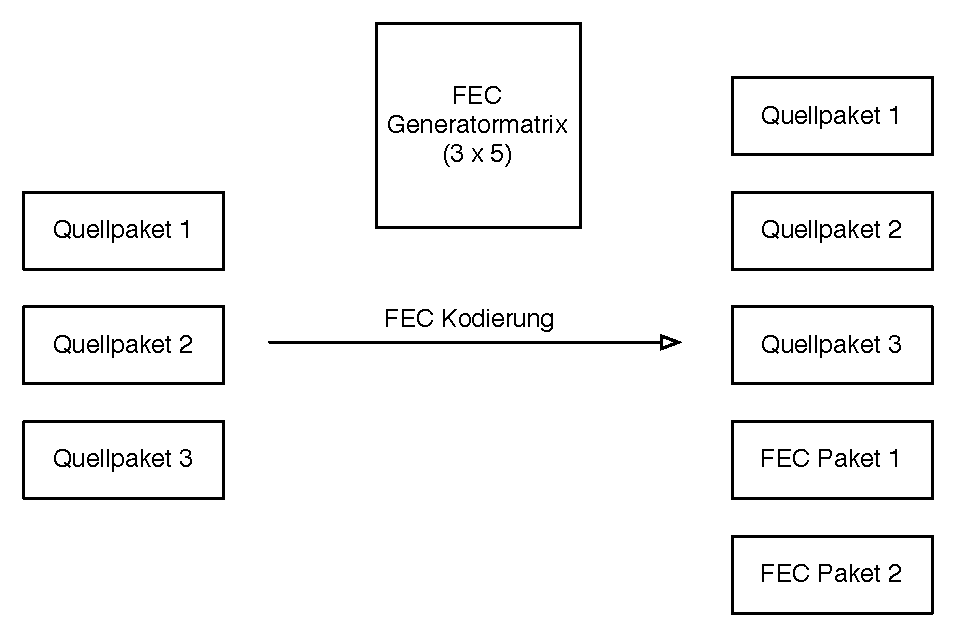
\includegraphics[scale=0.43]{feckodierung}
  \label{pic:feckodierung}
  \caption{Kodierung von Quelldaten}
\end{figure}

Zum Kodieren des $i$-ten Zielpaketes werden die $k$ Quellpakete mit
der $i$-ten Zeilen der Generatormatrix multipliziert und
dann summiert. Dazu wird das $j$-te Quellpakete mit der $j$-ten
Komponente der $i$-ten Zeilen multipliziert, so dass bei einer
systematischen Matrix, die die Einheitsmatrix enth�lt, die ersten $k$
Zielpakete dieselben Daten enthalten wie die ersten $k$ Quellpakete
(siehe Abb. \ref{pic:feckodierung}).

\subsection{Dekodieren von empfangenen Paketen}

\begin{figure}[htbp]
  \centering
  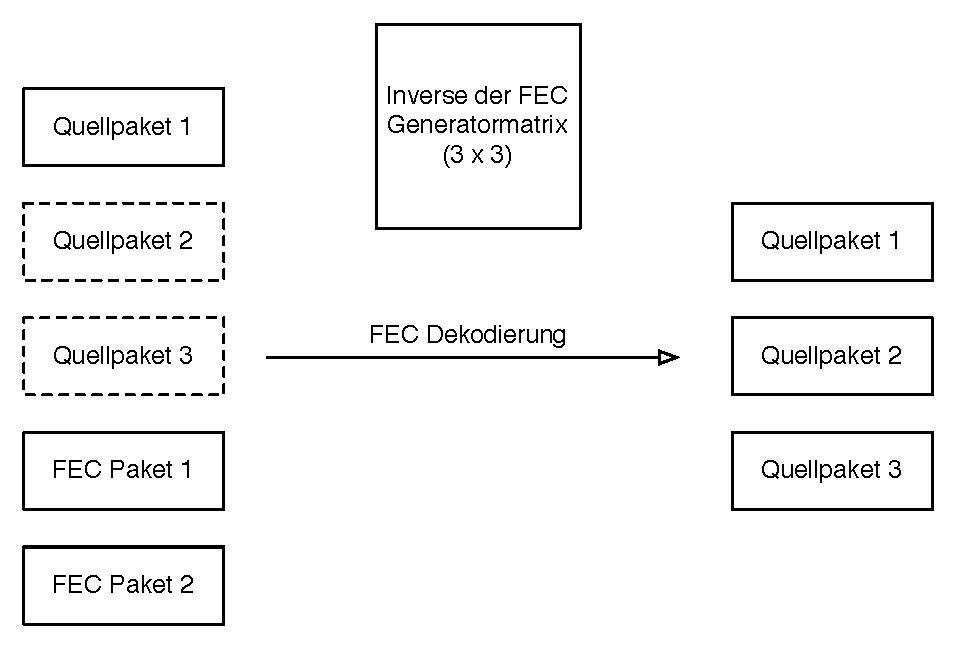
\includegraphics[scale=0.43]{fecdekodierung}
  \label{pic:fecdekodierung}
  \caption{Dekodieren von FEC-kodierten Daten}
\end{figure}

Zum Zur�ckgewinnen des $i$-ten Quellpaketes aus $k$ empfangenen
Paketen m�ssen die empfangenen Pakete mithilfe einer Untermatrix der
Generatormatrix dekodiert werden. Diese Dekodiermatrix wird berechnet,
indem die Zeilen die den Indexen der empfangenen Matrix entsprechen
aus der Generatormatrix in eine tempor�re $k \times k$ Matrix kopiert
werden, und diese invertiert wird. Werden jetzt analog zum
Kodierverfahren die empfangenen Daten an diese Matrix multipliziert,
gewinnt man die Quelldaten wieder (siehe Abb. \ref{pic:fecdekodierung}).

\section {Einsatz im Bereich MP3 Streaming}
\label{sec:fec-pkt}

Genau wie bei dem Verfahren in RFC 3119 sollten bei redundant
kodierten MP3-Daten ADUs verwendet werden, so dass bei einem
Paketverlust der nicht aufgehoben werden kann nicht gleich mehrere
MP3-Frames verloren gehen. Die eigentliche Fehlerkorrekturkodierung
erfolgt also nach dem Konvertieren der Eingangsframe in ADUs. Dazu
werden die ADUs in Gruppen von $k$ ADUs gesammelt, und aus denen dann
$n$ Pakete kodiert, die dann versendet werden k�nnen. Diese Gruppen
werden FEC-Gruppen genannt. Je nach Qualit�t des unterliegenden
Kommunikationsmedium k�nnen die Gr�ssen ($k$) dieser Gruppen und die
Anzahl der daraus kodierten Pakete ($n$) varieert werden, um ein gutes
Verh�ltnis zwischen benutzter Bandbreite und effektiver
Fehlerkorrektur zu erreichen.

\subsection{Verarbeitung von ADUs verschiedener L�nge}
Jetzt tritt allerdings ein anderes Problem auf. Im Gegensatz zu
MP3-Frames k�nnen ADUs verschieden lang sein (und sie es in der Praxis
auch immer). Das Verfahren von Rizzo kodiert allerdings nur
gleichlange Datenpakete. Man k�nnte die ADUs in einen langen
Datenpuffer zusammenh�ngen, und diesen Puffer dann in gleichgro�e
Pakete unterteilen, die redundant kodiert werden. Dieses Verfahren hat
allerdings den Nachteil, da� bei gr�sseren Paketverlusten, bei denen
die Quelldaten aus den empfangenen Daten nicht mehr hergestellt werden
k�nnen die ADUs der kompletten FEC-Gruppe verloren gehen. Da wir
jedoch ein systematisches FEC-Verfahren benutzen, k�nnen die ADUs mit
Nullen auf die Gr��e $l$ des gr��ten ADUs aufgef�llt werden, um somit
$n$ Pakete der L�nge $l$ zu kodieren, die ersten $k$ Pakete brauchen
aber jeweils nur der L�nge des entsprechenden ADUs zu sein, da sie auf
der Empf�ngerseite wieder mit Nullen aufgef�llt werden k�nnen. So
k�nnen bei gr��eren Paketverlusten immer noch die empfangenen Pakete
unter den $k$ ersten FEC-Paketen als MP3 ADUs benutzt werden (siehe
Abb. \ref{pic:fec-padding}).

\begin{figure}[htbp]
  \centering
  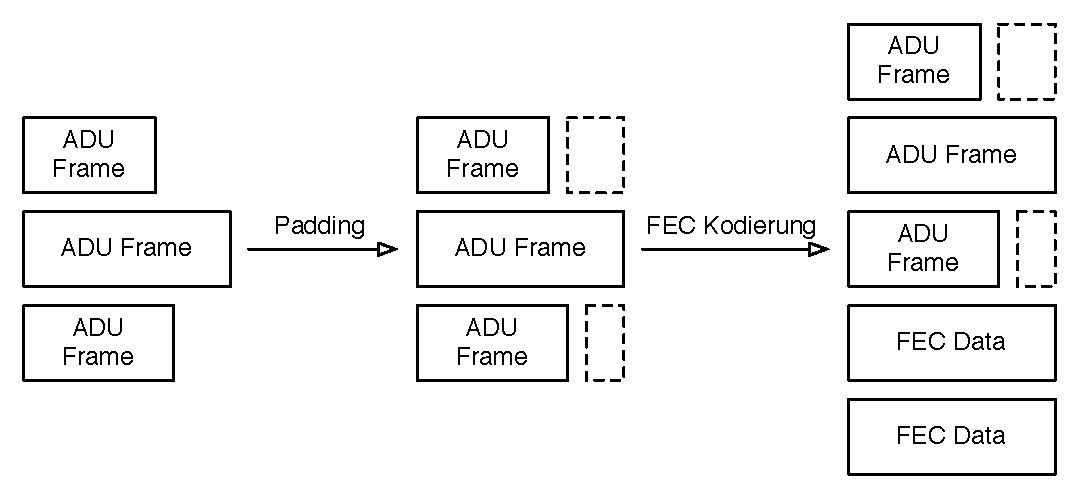
\includegraphics[scale=0.43]{fec-padding}
  \label{pic:fec-padding}
  \caption{Verarbeitung von ADUs verschiedener L�nge}
\end{figure}

\subsection{Protokoll zum Versenden von FEC-kodierten ADUs}

Zus�tzlich zu den eigentlichen FEC-kodierten Daten m�ssen bei dem Streamen
von FEC-kodierten MP3 ADUs wichtige Metainformationen �bermittelt
werden, wie z.B. die Sequenznummer des Pakets innerhalb der
versendeten Gruppe, die Sequenznummer der Paketgruppe, um bei
umgeordneten Paketen und bei Paketverlusten ankommende Pakete in die
richtige Gruppe zu ordnen, sowie ein Timestampfeld, um Aussetzer und
Synchronisationsprobleme des Stroms zu erkennen und handzuhaben.

\begin{figure}[htbp]
  \centering
  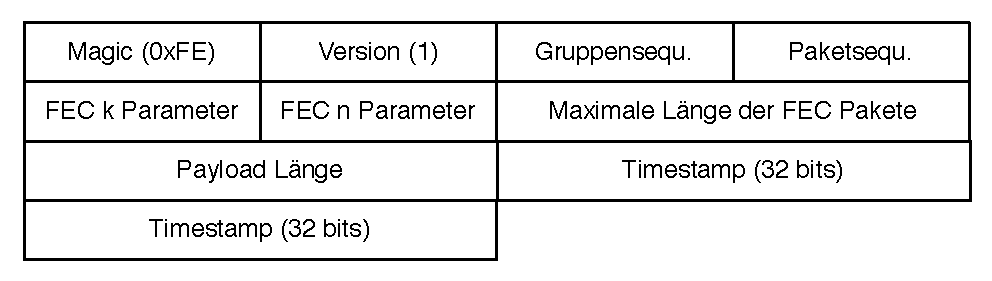
\includegraphics[scale=0.65]{fecpkt}
  \label{pic:fecpkt}
  \caption{Format des FEC-Paket Headers}
\end{figure}

% Gruppenbildung
Auf dem Empf�ngerseite werden die FEC-kodierten Daten anhand der
Sequenznummern in die richtigen FEC-Gruppen einsortiert. Ist beim
Abspielen einer FEC-Gruppe diese Gruppe nicht komplett empfangen
worden (d.h. es wurden weniger als $k$ Pakete von $n$ Paketen
empfangen), werden nur die empfangenen Pakete mit Paketsequenznummer
$< k$ ausgegeben (die wegen der systematischen Matrix gleich den
Eingangs-ADUs sind), so dass nicht die komplette FEC-Gruppe verloren
geht. Ist die Gruppe komplett empfangen worden, werden die
Eingangs-ADUs mit dem Verfahren von Rizzo wiederhergestellt und zu MP3
Frames konvertiert, und anschliessend ausgegeben.



\chapter{Implementierungs�bersicht}
\label{sec:implementation}

In diesem Kapitel wird die Struktur der implementierten Software
vorgstellt, sowie die Funktionsweise der einzelnen Programme erl�utert.
Anschliessend wird kurz �ber den Implementierungsvorgang eingegangen,
und letztendlich zuk�nftige Erweiterungen und Verbesserungen
vorgestellt.

% Struktur des Programms
\section{Struktur der implementierten Software}
\label{impl:struktur}

Die implementierte Software besteht aus mehreren kleinen Modulen, die
jeweils einen begrenzten Teil der Funktionalit�t implementieren. Diese
Module lassen sich in gr�ssere Gruppen einordnen:
\begin{itemize}
\item Datenstrukturen
\item Netzwerk
\item FEC
\item MP3
\end{itemize}

Die Module in der Datenstruktur-Gruppe sind von anderen Modulen unabh�ngig
und lassen sich auch in anderen Softwarepaketen
wiederverwenden. In dieser Gruppe sind folgende Module zu finden:
\begin{itemize}
\item Doppel verkettete Listen (siehe \ref{impl:dlist})
\item Bitvektore (siehe \ref{impl:bv})
\item Big-Endian Packing (siehe \ref{impl:pack})
\end{itemize}

In der zweiten Modulgruppe sind netzwerkrelevante Module zu finden:
\begin{itemize}
\item UDP Hilsfunktionen (siehe \ref{impl:network})
\item RTP Implementierung (siehe \ref{impl:rtp})
\end{itemize}

Die wichtigstes Modulgruppe beinhaltet Module zum Lesen und Schreiben
von MP3-Dateien, sowie zur Konvertierung von MP3-Frames in
ADUs. Zus�tzlich ist auch in einem gewissen Ma�e das Transkodieren von
MP3-Daten implementiert (Einlesen und Transformieren der Scalefactors
und der Huffmankodierten Daten). Dazu wurden die Algorithmen zum
Kodieren und Dekodieren von Huffmankodierten Daten in einem getrennten
Perlprogramm implementiert, das optimierten C Code produzieren kann.

Eine weitere wichtige Modulgruppe implementiert das
Fehlerkorrekturverfahren von Luigi Rizzo. Dazu ist eine
Implementierung von Galoisk�rper Arithmetik notwendig (hier nur f�r
\gf{2^8}). Zus�tzlich wird auch eine Implementierung von
Vandermondematrizen (Erstellen, Invertierung) ben�tigt.

Diese Modulgruppe wird durch die Implementierung des in Abschnitt
\ref{sec:fec-pkt} beschriebenen Protokolls erg�nzt, mit dem
FEC-kodierte ADUs gesendet und empfangen werden k�nnen.

% Aufteilung in Module
\section{Implementierte Module}
\label{impl:module}

% dlist
\subsection{Doppelt verkettete Listen}
\label{impl:dlist}

Doppelt verkettete Listen werden zum Puffern von einkommenden Paketen
bei den einzelnen Netzwerkclients benutzt, sowie zum Zwischenspeichern
von MP3-Frames bei der Konvertierung von MP3-Frames zu
ADUs. Zus�tzlich zu den notwendigen Routinen (Einf�gen, L�schen,
Initialisieren einer Liste, Freigeben einer Liste) sind auch
Suchfunktionen implementiert. Doppelt verkettete Listen bestehen aus
einem Listenkopf (\verb|dlist_head_t|), der Zeiger auf das erste sowie
auf das letzte Element der Liste speichert, und Listenknoten
(\verb|dlist_t|), die einen Zeiger auf ihr Datum, das naechste
Listenelement und das vorherige Listenelement speichern. Zur
Vereinfachung des Modulinterfaces werden auch \verb|dlist_push| und
\verb|dlist_pop| Funktionen zur Verf�gung gestellt.

% bv
\subsection{Bitvektor}
\label{impl:bv}

Das Bitvektormodul stellt Funktionen zur Verf�gung, mit der einzelne
Bits oder Bitgruppen aus einem Bytebuffer extrahiert werden
k�nnen. Die Gr�sse dieser Bitgruppen ist auf 32 Bits beschr�nkt, damit
diese auch in einem ``long'' zur�ckgegeben werden k�nnen. Die
Implementierung benutzt eine Datenstruktur, in der ein Zeiger auf den
Bytebuffer gespeichert wird, zus�tzlich zur Gesamtl�nge des
Bytebuffers (in Bits) und einem Indexzeiger, der auf die noch
ungelesene (ungeschriebene) Bits zeigt. Geschrieben wird mit der
\verb|bv_put_bits| Funktion, gelesen mit der \verb|bv_get_bits|
Funktion. Der Bytebuffer wird so gehandhabt, das schwergewichtigere Bits
(die in dem Byte also einen gr�sseren numerischen Wert kodieren)
zuerst gelesen (oder geschrieben) werden.

Dieses Modul wird beim Einlesen von RTP-Paketen und beim Einlesen und
Konvertieren von MP3-Daten benutzt.

% pack
\subsection{Bigendian Packing}
\label{impl:pack}

Dieses Modul stellt mehrere Funktionen zum Packen und Entpacken von
Bigendiandaten.

% network
\subsection{Netzwerk Hilfefunktionen}
\label{impl:network}

In diesem Modul sind einfache Wrapperfunktionen um die unterliegenden
BSD Socket API implementiert, die die Implementierung der
Streamingclients und Streamingserver vereinfacht. Es werden die
Funktionen \verb|net_udp_recv_socket|, das ein horchendes UDP Socket
erstellt, und \verb|net_udp_send_socket|, das ein sendendes UDP Socket
erstellt, zur Verf�gung gestellt. Falls das Socket auf eine
Multicast-Adresse gebunden wird, wird die TTL auf einen �bergebenen
Wert gesetzt, und Mitgliedschaft im Multicast-Netz angemeldet (f�r ein
horchendes Socket).

% rtp
\subsection{RTP Schicht}
\label{impl:rtp}

In diesem Modul wird das Erstellen, Einlesen und Senden von
RTP-Paketen (RTP version 2 \cite{RFC1889}) implementiert. Aufbauend
auf diesen Funktionen wird auch das Erstellen, Einlesen, Senden und
Signieren von RTP Pakete mit MP3 Nutzdaten implementiert
(\cite{RFC2250}, \cite{RFC3119}). Diese Funktionen werden von den
RFC-2250 und RFC-3119 Clients und Server benutzt. Der
Synchronisationsquelleidentifikator und die
Inhaltsquellenidentifikatore werden auf $0$ gesetzt und werden auch
beim Einlesen einfach ignoriert. Fragmentierung bei RFC-2250 wird auch
nicht unterst�tzt, da UDP Pakete lang genug sind, um die l�ngsten
MP3-Frames ohne Fragmentierung zu senden.  Sendefunktionen
(\verb|rtp_*_send|), Packfunktionen (\verb|rtp_*_pack|),
Empfangsfunktionen (\verb|rtp_*_read|) und Entpackfunktionen
(\verb|rtp_*_unpack|) werden zur Verf�gung gestellt.  Die
Lesefunktionen lesen von einem UDP Socket.

% mp3
\subsection{MP3}
\label{impl:mp3}

Das MP3-Modul besteht eigentlich aus mehreren Modulen. Die Strukturen,
die zur Handhabung von MP3-Da\-teien, MP3-Frames und ADUs notwendig sind
werden in einer Header-Datei definiert, die von den verschiedenen
Modulen verwendet wird. Das erste Modul liest MP3-Frames aus
MP3-Dateien, extrahiert allerdings nur die Header-Struktur. Das zweite
Modul liest die eigentlichen kodierten Daten aus den MP3-Frames 
(Skalierungsfaktoren, Huffmankodierte Daten, Seiteninformation). Das
letzte Modul kann diese extrahierte Information wieder serialisiert
zur�ckschreiben.

Das MP3-Modul benutzt eine Datenstruktur zur Darstellung von
MP3-Dateien (\verb|mp3_file_t|), in der der Dateideskriptor, die
Gr�sse der Datei und der jetzige Offset innerhalb der Datei
gespeichert werden.  Beim Lesen von MP3-Daten werden nicht konforme
Daten (ohne Synchronisationsheaderfeld) maximal \verb|MP3_MAX_SYNC|
mal �bersprungen, was bei l�ngeren ID3-Headern (z.B. bei eingebetteten
Bildern) zu Probleme f�hren kann. Eine m�gliche Erweiterung w�r das
Speichern der ID3-Daten in der MP3-Datei-Struktur.

MP3-Frames werden durch die Funktion \verb|mp3_next_frame| in die
\verb|mp3_frame_t| Struktur eingelesen, in der auch die
Headerinformationen durch die Funktion \verb|mp3_read_hdr| extrahiert
werden. Die Rohdaten aus der MP3-Datei werden in der MP3-Frame
Struktur in den Rohdatenpuffer \verb|raw| eingelesen.
Seiteninformation (Sideinformation) wird in die Strukturen
\verb|mp3_si_t| (allgemeine Seiteninformation), \verb|mp3_channel_t|
(Stereokanalinformation) und \verb|mp3_granule_t| (Granuleinformation)
durch die Funktion \verb|mp3_read_si| eingelesen. Diese Information
kann durch die Funktionen \verb|mp3_fill_hdr| und \verb|mp3_fill_si|
wieder in den Rohdatenpuffer der MP3-Frame Struktur zur�ckserialisiert
werden. Dieser Rohdatenpuffer kann mit der Funktion
\verb|mp3_write_frame| in eine MP3-Datei geschrieben werden.

Diese Module werden von dem MP3 nach ADU Konvertierungsmodul und von
den einzelnen Client- und Serverprogrammen benutzt (nicht aber von dem
RFC-2250 Client, der die RTP-Nutzdaten uninterpretiert ausgibt).

% aq
\subsection{MP3 nach ADU Konvertierung}
\label{impl:aq}

In diesem Modul werden die in Abschnitt \ref{sec:aq} beschriebenen
Algorithmen implementiert, mit dem MP3-Frames nach ADUs konvertiert
werden k�nnen. Dazu wird die Datenstruktur \verb|aq_t| benutzt, die
zwei verkettete Listen speichert, eine Liste von MP3-Frames und eine
Liste von ADUs. Dabei ist die Datenstruktur f�r ADUs, \verb|adu_t|,
dieselbe wie f�r MP3-Frames. Wenn MP3-Frames nach ADU konvertiert
werden, werden sie mit der Funktion \verb|aq_add_frame| in die
MP3-Frame Liste eingef�gt. Sind gen�gend MP3-Frames vorhanden, um ein
ADU zu produzieren, gibt diese Funktion den R�ckgabewert $1$ zur�ck,
sonst $0$. Mit \verb|aq_get_adu| kann dann das konvertiert ADU aus der
ADU-Liste extrahiert werden. Bei der Konvertierung von ADUs nach
MP3-Frames wird mit den Funktionen \verb|aq_add_adu| und
\verb|aq_get_frame| �hnlich vorgegangen.

Das Konvertierungsmodul wird von den RFC-3119 Client- und
Serverprogrammen benutzt, sowie als Teil des FEC Kodierungsprozess in
den FEC Client- und Serverprogrammen.

% galois
\subsection{Galois K�rper Arithmetik}
\label{impl:galois}

Um eine Erh�hung der Kodierungsl�nge von FEC-Koeffizienten bei
Multiplikationsvorg�ngen wird bei dem FEC-Verfahren von Luigi Rizzo in
einem endlichen K�rper gerechnet. Bei dem FEC-Verfahren, das im Rahmen
dieser Studienarbeit implementiert wurde, wird in dem Galoisk�rper
\gf{2^8} gerechnet. Addition (was dieselbe Operation wie Substraktion
ist) wird mit $XOR$ implementiert, Multiplikation und Division mittels
Lookuptabellen. Diese Tabellen werden mit der Funktion \verb|gf_init|
initialisiert, wobei das primitive Polynom $x^8 + x^4 + x^3 + x^2 + 1$
benutzt wird. Ein Element in \gf{2^8} wird mit der Datenstruktur
\verb|gf| dargestellt. Arithmetische Operationen sind keine
Funktionen, sondern Makros: \verb|GF_ADD|, \verb|GF_MUL| und
\verb|GF_INV|.

Das Galoisarithmetikmodul wird von dem Matrixmodul und dem FEC-Modul
benutzt.

% matrix
\subsection{Vandermondematrix Arithmetik}
\label{impl:matrix}

In diesem Modul wird Matrixarithmetik f�r $GF(2^8)^{m \times n}$
Matrizen implementiert. Eine Matrix ist ein Array von \verb|gf|
Elementen. Mit der Funktion \verb|matrix_mul| werden Matrizen
multipliziert, mit \verb|matrix_inv| werden Matrizen mit dem
Gauss-Jordan Verfahren invertiert, und als spezielle Optimierung
k�nnen Vandermonde Matrizen mit \verb|matrix_inv_vandermonde|
invertiert werden. In dem vorliegenden Quellcode von Luigi Rizzo
verbarg sich in dieser Funktion ein Fehler, der allerdings bei dem
FEC-Verfahren nicht zum Vorschein kam, weil die benutzte
Vandermonde-Matrix eine spezielle Form hatte, die den Fehler nicht
ausl�ste. Zur Vereinfachung des Quellcodes wurde im Galoisarithmetik
eine spezielle Funktion \verb|gf_add_mul| implementiert, die eine
Matrixspalte $a$ multipliziert mit einer Konstante $c$ auf eine
Matrixspalte $b$ addiert.

Das Matrixarithmetikmodul wird von dem FEC-Modul zum Kodieren und
Dekodieren von FEC-Daten benutzt.

% fec
\subsection{Vorw�rtsfehlerkorrektur (FEC)}
\label{impl:fec}

In diesem Modul wird das Fehlerkorrekturverfahren, dass von Luigi
Rizzo entworfen wurde implementiert. FEC-Parameter $k$ und $n$, sowie
die Generatormatrix werden in der Datenstruktur \verb|fec_t|
gespeichert. Diese Struktur wird mit der Funktion \verb|fec_new|
alloziiert und initialisiert, und sp�ter mit der Funktion
\verb|fec_free| wieder freigegeben. Zur Kodierung wird die Funktion
\verb|fec_fencode| benutzt, die zu Quelldaten ein bestimmtes Zielpaket
$i$ mit $i < n$ produziert. Quelldaten werden als Arrays von Pointer
auf \verb|gf| Daten �bergeben, das Zielpaket ist ein Array von
\verb|gf| Elementen. Zur Dekodierung wird die Funktion
\verb|fec_decode| benutzt, die zu einem Array von kodierten Pakete und
einem Array von Indexen die Quelldaten wiederherstellt. Die Indexe der
kodierten Pakete wird nicht in den kodierten Paketen selbst kodiert,
sondern muss getrennt �bermittelt. Bei dem implementierten FEC
Protokoll wird diese Information in dem UDP Paket Header �bermittelt.

Das FEC-Modul wird von den FEC Client- und Serverprogrammen verwendet.

% FEC pkt
\subsection{FEC Protokoll}
\label{impl:fec-pkt}

In diesem Modul wird das in Abschnitt \ref{sec:fec-pkt} beschriebene
Protokoll implementiert. FEC-Pakete werden in der Struktur
\verb|fec_pkt_t| gespeichert, Headerdaten in der Struktur
\verb|fec_pkt_hdr_t|. Wie bei dem RTP-Modul werden Funktionen zum
Senden und Lesen von FEC-Paketen zur Verf�gung gestellt. Im Gegensatz
zu dem RTP-Modul werden Headerfelder nicht automatisch hochgez�hlt
beim Senden von Paketen, da es kein lineares Sequenznummernfeld gibt.

Diese Modul wird von den FEC-Netzwerkprogrammen benutzt.

\section{Implementierte Programme}
\label{impl:programme}

In diesem Abschnitt werden die implementierten Programme vorgestellt,
ihre Funktionsweise erkl�rt und die Benutzerschnittstelle sowie
Einsatzbereiche kurz vorgestellt.

% poc-http
\subsection{HTTP Streaming Server}
\label{impl:poc-http}

Es wurden zwei Versionen des HTTP Streaming Servers implementiert. Die
erste Version wird �ber einen Internet Server wie inetd oder tcpserver
aufgerufen, liest die einkommenden Daten von dem Standardeingabestrom
(stdin), und schreibt die MP3-Datei auf den Standardausgabestrom. Die
MP3-Daten, die versendet werden sollen werden �ber RTP empfangen. Die
urspr�ngliche Idee bei dem Server war, RTP Multicast Str�me an
konventionelle MP3-Clients zu senden. Diese Implementierung benutzt
die \verb|poll| Funktion, so da� sie nur bedingt portabel ist.

Die zweite Implementierung des HTTP Server gleicht eher dem Ansatz der
anderen MP3-Streaming Server, und liest seine Daten aus einer Liste
von Dateien (oder von der Standardeingabe). Diesmal wird kein Internet
Server ben�tigt, da das Annehmen von Verbindungen von dem Server
selbst verwaltet wird. Dieser Server benutzt die \verb|select| API,
die der BSD Socket API geh�rt, so dass diese Implementierung auf
Systemen, die die BSD Socket API unterst�tzen portabel sein sollte.

Die Unterst�tzung des HTTP Protokolls beschr�nkt sich auf das
Notwendigste. Es wird eine maximale Headerl�nge vorausgesetzt. Ist
innerhalb dieser L�nge kein Headertrenner zu finden (zweimal
\verb|\r\n|, so wird die Anfrage verworfen. Als einzige Anfrage wird
\verb|GET /| unterst�tzt, auf die der Server die MP3-Daten
zur�ckschickt. Alle andere Anfragen werden verworfen. Der HTTP Server
synchronisiert die Senderate mit der Abspielrate der MP3-Daten,
anstatt sich auf die Synchronisierung durch den Empf�nger zu verlassen
(was bei einem einzelnen Client noch vertretbar ist, bei mehreren
Clients allerdings zu Problemen f�hren kann, wenn Clients
unterschiedliche Pufferverfahren haben). Bei der ersten
Implementierung wird auf Synchronisierung ganz verzichtet, da diese
durch den RTP Server angegeben wird.

Durch das Einlesen von einzelnen MP3-Frames und das Extrahieren der
Headerinformation ist es m�glich, MP3-Daten mit variabler
Bitratenkodierung zu versenden, was von den meisten HTTP MP3
Streamingservern nicht unterst�tzt wird.

% poc-2250
\subsection{RFC-2250 Streaming Server}
\label{impl:poc-2250}

Der RFC-2250 MP3-Streaming Server \verb|poc-2250| liest MP3-Frames aus
mehreren MP3-Dateien (oder von der Standardeingabe), und verschickt
jedes einzelne Frame als Nutzdaten eines RFC-2250 Pakets. Dabei
wird die Zeit innerhalb der MP3-Datei als RTP-Timestamp verwendet.
Alternativ k�nnen die RTP Pakete signiert werden, indem das Verfahren
aus Abschnitt \ref{sec:rtp-sec} verwendet wird. Nachdem ein Paket
gesendet wurde synchronisiert der Server sich auf den MP3-Strom, und
wartet solange bis das n�chste Frame der Datei zeitlich abgespielt
werden muss, um das neue Paket abzuschicken. Bei dem Aufrufen des
Servers kann zus�tzlich noch die Lebensdauer (TTL) von
Multicastpaketen eingestellt werden, um den Verbreitungsgrad des MP3
Stroms zu kontrollieren.

% pob-2250
\subsection{RFC-2250 Streaming Client}
\label{impl:pob-2250}

\verb|pob-2250| ist das Clientpendant zum RFC-2250 Server. Der
Client empf�ngt RTP-Pakete, indem er ein UDP Socket �ffnet und davon
liest. Einkommende Pakete werden in eine Pufferliste einsortiert,
doppelte Pakete verworfen, und nach einer bestimmten Pufferzeit wird
die Liste abgearbeitet und die Nutzdaten der gepufferten RTP-Pakete an
den MP3-Dekodierer weiteregeleitet, indem sie auf der Standard Ausgabe
ausgegeben werden. Falls die einkommenden Pakete signiert sind, wird
ihre G�ltigkeit mit dem Serverzertifikat �berpr�ft. Statistiken �ber
einkommende Pakete werden in der \verb|pob_stat_t| Struktur
festgehalten:
\begin{itemize}
\item Anzahl der empfangenen Pakete
\item Anzahl der Pakete, die in der falschen Reihenfolge waren
\item Anzahl der nicht dekodierbaren Pakete
\item Anzahl der nicht oder falsch zertifizierten Pakete, falls SSL
  benutzt wird
\item Anzahl der �berl�ufe des Puffers
\item Anzahl der Unterl�ufe des Puffers
\end{itemize}

\verb|pob-2250-rb| ist eine verbesserte Version von \verb|pob-2250|,
die Ringpuffer zum Puffern von einkommenden Daten verwendet.

% poc-3119
\subsection{RFC-3119 Streaming Server}
\label{impl:poc-3119}

Der RFC-3119 Streaming Server \verb|poc-3119| ist im Aufbau
\verb|poc-2250| sehr �hnlich. Allerdings werden nach dem Einlesen
MP3-Frames erst nach ADUs konvertiert, indem sie in eine \verb|aq|
Struktur eingespielt werden. Ist ein ADU produziert worden, wird es in
ein RFC-3119 Paket gespeichert und versendet. Nach dem Versenden
einer ADU synchronisiert sich der Server wie \verb|poc-2250| auf den
gelesenen MP3-Strom. Die Interleaving Funktion von RFC-3119 wird noch
nicht unterst�tzt. Dazu m�ssten die ADUs nicht sofort versendet
werden, sondern erst in Gruppen gespeichert werden, die vor dem
Versenden umsortiert werden. Wie bei \verb|poc-2250| k�nnen auch hier
Pakete signiert werden und eine Multicast Lebenszeit angegeben werden.

% pob-3119
\subsection{RFC-3119 Streaming Client}
\label{impl:pob-3119}

Der RFC-3119 Streaming Client \verb|pob-3119| ist im Aufbau dem
\verb|pob-2250| Client identisch, bis auf den Unterschied, dass die in
den empfangenen Pakete enthaltenen ADUs erst wieder zur�ck nach
MP3-Frames konvertiert werden, bevor sie dem MP3-Dekodierer �ber die
Standardausgabe gegeben werden. Bei fehlenden ADUs werden leere ADUs
eingef�gt, die die Korrektheit des MP3-Stromes wiederherstellen (also
gen�gend Platz zur Verf�gung stellen, um das Bitreservoir des n�chsten
korrekt empfangenen MP3-ADUs zu speichern). Falls der RFC-3119 Client
mit dem MP3-Dekodierer integriert wird w�re diese R�ckwandlung nach
MP3-Frames nicht notwendig, da der Dekodierer mit ADUs umgehen
kann. Im Fall von Paketverlusten k�nnte der Dekodierer einfach Pausen
in den dekodierten Strom einf�gen. Die Interleaving Funktion von
RFC-3119 wird auch im Client noch nicht vollst�ndig unterst�tzt,
empfangene Pakete werden allerdings innerhalb der Pufferzeit in die
richtige Reihenfolge gebracht (und nicht bis ein Paket der n�chsten
Gruppe empfangen wird), so dass RFC-3119 Streams mit Interleaving
korrekt dekodiert werden.

\verb|pob-3119-rb| ist eine verbesserte Version von \verb|pob-3119|,
die Ringpuffer zum Puffern von einkommenden Daten verwendet.

% poc-fec
\subsection{FEC Streaming Server}
\label{impl:poc-fec}

Der FEC Streaming Server \verb|poc-fec| ist im Aufbau den andere
Streaming Servern sehr �hnlich. Wie bei \verb|poc-3119| werden die
eingelesenen MP3-Daten zuerst nach ADUs konvertiert, um anschliessend
in FEC-Gruppen von $k$ Paketen gruppiert zu werden. Diese FEC Gruppen
werden zu $n$ Paketen redundant kodiert, und in regelm�ssigen
Abst�nden versendet. Unter diesen $n$ Paketen sind wegen der
systematischen Matrix die $k$ Eingangs-ADUs.

% pob-fec
\subsection{FEC Streaming Client}
\label{impl:pob-fec}

Der FEC Streaming Client \verb|pob-fec| ist im Aufbau dem
\verb|pob-3119-rb| Client �hnlich. Allerdings werden bei
\verb|pob-fec| einkommende Pakete erst in FEC-Gruppen einsortiert, die
anschliessend dekodiert werden. Anschliessend werden die FEC-Gruppen
mit dem FEC-Verfahren von Rizzo nach ADUs dekodiert, die anschliessend
nach MP3-Frames konvertiert werden. Bei fehlenden Paketen werden
systematisch �bertragene Pakete direkt nach MP3-Frames konvertiert, so
dass der Paketverlust minimiert wird. Anschliessend werden die
MP3-Frames dem MP3-Dekodierer �bergeben.

% mp3cue
\subsection{MP3-CUE Dateien Parser}
\label{impl:mp3cue}

Die implementierten Module wurden auch benutzt um Softwarewerkzeuge
herzustellen, die nicht direkt mit dem Streamen von MP3-Daten zu tun
haben. So wurde ein Werkzeug implementiert, mit dem MP3-Dateien
geschnitten werden k�nnen (an Framegrenzen, bzw. an ADU
Grenzen). Dieses Werkzeug liest ``CUE'' Dateien ein, die angeben, wie
eine l�ngere MP3-Datei in einzelne Einheiten (zum Beispiel
Musikst�cke) gegliedert ist, und welchen Namen diese Einheiten
tragen. Das Werkzeug benutzt einen Yacc-Parser, um ``CUE'' Dateien
einzulesen, und benutzt die in Abschnitt \ref{sec:transcoding}
vorgestellten Algorithmen, um eine saubere Trennung von einzelnen
Einheiten zu erreichen.

\section{Implementierungsvorgang}

Die oben beschriebene Software wurde in mehreren Schritten
implementiert. Die erste Version, die nur einen einfachen RFC-2250
Streamserver und -client enthielt, wurde HP/UX 10.20 (PA-RISC
Architektur, HP ANSI C Compiler) implementiert, und sollte HTTP
Streams aus dem Internet in einem lokalen Netzwerk �ber Multicast
weitersenden. Aufbauend auf diesen Server wurde eine rudiment�re und
fehlerhafte Implementierung von RFC 3119 programmiert, und die gesamte
Software unter Linux und Freebsd portiert (der Aufwand war relativ
gering). Ein Plugin f�r den Audioplayer XMMS, das RFC-2250 Daten
empfangen konnte, wurde auch implementiert.

Die zweite Version der Software wurde 8 Monate sp�ter im Rahmen dieser
Studienarbeit implementiert. Dabei wurde von Anfang an Wert auf
Portabilit�t und Sauberkeit gelegt. Die einzelnen Module wurden sauber
getrennt, alle grundlegende Module (Datenstrukturen,
Galoisfeldarithmetik, Matrixarithmetik) wurden mit eigenen
Testprogrammen getestet (diese Testprogramme kann man kompilieren
indem bestimmte Flags im Makefile aktiviert werden). Mit diesen Tests
wurde auch ein Fehler in der Implementierung der Vandermonde
Matrixarithmetik von Luigi Rizzo selbst gefunden, die allerdings auf
sein Verfahren keinen Einfluss hatte, da die erste Zeile seiner
Vandermondematrizen immer aus Potenzen von $0$ bestand.

Die Module wurden ausf�hrlich dokumentiert, und �hnlich dem ``Literate
Progamming'' von Donald Knuth kann aus dem Quellcode eine formatierte
Quellcodedokumentation generiert werden. Dazu wird das Programm
\verb|texify| eingesetzt, das auf eine Implementierung von Thomas
Fuhrmann basiert, jedoch leicht ver�ndert wurde.

Bestimmte Module (Datenstrukturen, Galoisarithmetik) wurden mit dem
Programm \verb|clint| �berpr�ft, dieser Ansatz wurde aber nach einer
bestimmten Zeit verworfen, da die Ver�nderungen zum Eliminieren von
\verb|clint|-Warnungen zum grossen Teil nur kosmetische waren, und
schwerwiegendere Fehler meistens durch den Compiler schon abgefangen
wurden. \verb|NULL|-Pointer Fehler, korrupte Datenstrukturen und
schwerwiegende Betriebssystemfehler (z.B. Fehler bei der Alloziierung
von Arbeitsspeicher) wurden durch Assertions abgefangen, die im Moment
f�r ein ``sicheres'' Abfangen von Fehlern noch notwendig sind.

Da weder Probleme mit Memory Leaks oder intensiver CPU-Nutzung bemerkt
wurden, wurde vorerst auf den Einsatz von Profilierungswerkzeugen verzichtet.



\chapter{Zusammenfassung}
\label{sec:zusammenfassung}

\section{Schlussfolgerungen}
\label{sec:schlussfolgerung}
In dieser Studienarbeit wurden die existierenden Verfahren zum
Streamen von MP3-Daten vorgestellt, sowie auf ihre Vorteile und
Nachteile eingegangen.

Alle Verfahren wurde nachimplementiert, so dass sie auch in der Praxis
getestet werden konnten. Zwei dieser Verfahren, die MP3-Daten �ber RTP
versenden, wurden erweitert um ein sicheres Versenden von MP3-Daten zu
er\-m�\-gli\-chen (es ist einem Angreifer nicht mehr m�glich, fremde
MP3-Daten in einen MP3-Strom einzuf�gen). Die entwickelten
Softwaremodule konnten auch anderweitig eingesetzt werden, um ein
Werkzeug zum sauberen Schneiden von MP3-Dateien zu realisieren.

Weiter wurde ein Protokoll entworfen, mit dem MP3-Daten redundant
kodiert und versendet werden k�nnen, um Aussetzer bei Paketverlusten
im unterliegenden Kommunikationsmedium (hier UDP) zu vermeiden. Dieses
Protokoll wurde auch implementiert, indem das paketbasierte
FEC-Verfahren von Luigi Rizzo verwendet wurde.

\section{M�gliche Erweiterungen}
\label{sec:erweiterungen}
Das urspr�ngliche Ziel dieser Studienarbeit war die Implementierung
einer autoadaptiven Fehlerkorrektur f�r MP3-Streaming. Bei erh�hter
Redundanzkodierung sollten die MP3-Daten niederskaliert werden, um die
Netzwerkbelastung in Grenzen zu halten. Allerdings war die
Implementierung eines MP3-Transkodierers zu aufwendig, da die
Dokumentation zu dem MP3-Format sehr sp�rlich ist, und das Debuggen
solcher Funktionalit�ten sehr schwer zu gestalten ist. Weiterhin war
das vorgeschlagene Verfahren, die Huffmankodierten Daten des MP3
Stromes runterzukodieren zu ungenau, um eine bestimmte Zielbitrate zu
erreichen. Ein praktischerer Ansatz w�re gewesen, einen existierenden
MP3-Encoder zu benutzen, der als Eingangsdaten einen MP3-Strom
benutzen kann. Mittlerweile kann die Lame Softwarebibliothek
MP3-Str�me umskalieren, so dass im Grunde genommen der Implementierung
einer autoadaptiven Fehlerkorrektur mit Transkodierung des MP3-Stromes
nichts im Wege steht.

Weiterhin ist das offene Vorbis Format sehr einfach handzuhaben, und
unterst�tzt auch ``Bitpeeling'', d.h. die M�glichkeit, Teile eines
Frames wegzulassen ohne die Dekodierbarkeit der Audiodaten zu
gef�hrden (es wird nur ein Qualit�tsverlust in Kauf genommen). Mit
diesem Verfahren lassen sich die Audiodaten ohne intensive Rechnungen
an die Netzwerkbandbreite anpassen. Das Vorbis Format benutzt auch
unabh�ngige ADUs als Frames, so dass die Konvertierung von Frames nach
ADUs wegf�llt. Mittlerweile wurde ein HTTP-Vorbis Streamer
implementiert.

Die Paketverlustrate �ndert sich meistens rasch, so dass eine
statische Einstellung der Fehlerkorrekturparameter nicht vertretbar
ist. Dazu m�sste im Fall von Multicast Streaming ein Feedbackprotokoll
benutzt werden, um die Fehlerkorrektur den W�nschen der meisten
Clients anzupassen. Dazu k�nnte man einer der vielen vorgeschlagenen
Feedbackprotokolle benutzen. Weiterhin sollten die Netzwerkprogramme
auf IPv6 portiert werden.

Letztendlich gibt es bei der implementierten Software noch viele
L�cken, wie z.B. eine gute Ausnahmebehandlung. In den meisten F�llen
wird im Moment bei schwerwiegenden Fehlern einfach der Prozess
quittiert.


\newpage
\addcontentsline{toc}{chapter}{\bibname}
\nocite{*} 
\bibliographystyle{itmalpha}
\bibliography{studienarbeit}

\appendix

\chapter{Code}
\label{sec:code}
\lstset{
  language=C,
  basicstyle = \small,
  columns = fullflexible,
  xleftmargin = 6mm,
  xrightmargin = 6mm,
  stringstyle = \textsl,%\itshape,
  showstringspaces = false,
  numbers = left,
  stepnumber = 1,
  numberstyle = \tiny,
  captionpos = b
}

\include{pack}
\include{dlist}
\include{network}
\include{bv}
\include{mp3}
\include{aq}
\include{rtp}
\include{galois}
\include{matrix}

\include{fec}
\include{fec-pkt}
\include{fec-group}

\include{rtp-rb}
\include{fec-rb}


\include{poc-http}
\include{poc-2250}
\include{pob-2250}
\include{pob-2250-rb}

\include{poc-3119}
\include{pob-3119}
\include{pob-3119-rb}

\include{poc-fec}
\include{pob-fec}

\include{ogg}
\include{pogg-http}

%\chapter{Fehlerlogbuch}

%\include{errorlog}

\end{document}
